\chapter{Graph Parsing}

\section{Algorithm}

\tikzset{% 
  not allowed/.style={%
    dotted,
    very thick,
    color=red
  }
}
\tikzset{% 
  required/.style={%
  }
}
\tikzset{% 
  optional/.style={%
    dashed
  }
}
\tikzset{% 
  pointO/.style={%
    fill=black,regular polygon, regular polygon sides=4,inner sep=1pt
  }
}
\newlength\vertSmall
\newlength\vertBig
\newlength\vertBigger
\newlength\labelGap
\newlength\coordGap

\newenvironment{tightflushright}{
  \null\hfill
}{
}

\subsection{Parsing Algorithm for Graphs}

% TODO - Add the intuition that when edges are added to/from the external point
% to the span, those edges are all going to be crossed at some point in the
% future.

In this section we sketch our algorithm, focusing on how it differs from \textcite{ec}'s tree parsing algorithm.
For the full derivation see the supplementary material.

The algorithm is a dynamic program defined by (1) a set of items, and (2) deduction rules that define how an item can be composed from other items.
To make the deduction rules manageable, we define some constraints explicitly, and then use code to enumerate all options and enforces additional constraints.
The representation described above requires directed, labeled edges, and spines.
To simplify the presentation of the algorithm we first focus on deduction rules for undirected, unlabeled edges and ignore spines, then return to these later.

To enable efficient parsing we restrict the space we consider, not covering a few specific one-endpoint-crossing structures as described earlier.
In practice, these structures are rarely observed in the PTB, and when they do occur it is usually due to where punctuation attaches.

\paragraph{Notation}
We use $p$, $q$, etc to refer to word positions.
To indicate ranges we use $[pq]$, $[pq)$, $(pq]$, or $(pq)$, where the bracket variations indicate inclusion, $[]$, or exclusion, $()$, of the endpoint.
To indicate an edge we use two points without brackets, \myeg $pq$.
To define a class of edges we either use a point and a set connected by a dash, \myeg $o$--$(pq)$, or two sets connected by a dash, \myeg $(ps)$--$(sq)$.

\subsubsection{Item Types}

Rather than the conventional constituency parsing approach where items fully cover words and end in the gaps between words, our items fully cover the gaps and end on the words, as shown in Figure~\ref{fig:alg-example}, and like in \textcite{eisner-satta-1999}'s algorithm.
We use six item types, differing in the type of edge crossing they contain.  \\

\hspace{-8mm}
\begin{tabular}{l@{\hskip 3pt}l}
  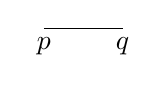
\begin{tikzpicture}
    \node (p) at (0.5, 0) {$p$};
    \node (q) at (1.5, 0) {$q$};
    \draw (p.north) -- (q.north);
  \end{tikzpicture} &
  \parbox{0.36\textwidth}{
    \textbf{$I$, Interval}
    A span in which all points in $(pq)$ have a parent in $[pq]$, and no edges exist that go from outside $[pq]$ to points in $(pq)$. \\
  } \\
  \begin{tikzpicture}
    \node (p) at (0, 0) {};
    \node (q) at (1, 0) {};
    \node (o) at (1.5, 0) {$o$};
    \draw (p.north) -- (q.north);
    \draw [out=45,in=135] (p.north) to (o.north);
  \end{tikzpicture} &
  \parbox{0.36\textwidth}{
    \textbf{$X$, Exterval}
    An interval plus a single edge between $o$ and either $p$ or $q$, where $o$ is outside $[pq]$. \\
  } \\
  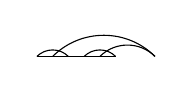
\begin{tikzpicture}
    \node (p) at (0, 0) {};
    \node (m1) at (0.2, 0) {};
    \node (m2) at (0.4, 0) {};
    \node (m3) at (0.6, 0) {};
    \node (m4) at (0.8, 0) {};
    \node (q) at (1, 0) {};
    \node (o) at (1.5, 0) {};
    \draw (p.center) -- (q.center);
    \draw [out=45,in=135] (m1.center) to (o.center);
    \draw [out=45,in=135] (m4.center) to (o.center);
    \draw [out=45,in=135] (p.center) to (m2.center);
    \draw [out=45,in=135] (m3.center) to (q.center);
  \end{tikzpicture} &
  \parbox{0.36\textwidth}{
    \textbf{$B$, Both}
    An interval $[pq]$ and a point $o$.
    $o$--$(pq)$ edge may be crossed by $p$--$(pq)$ or $q$--$(pq)$ edges, and at least one crossing of each type occurs. \\
  } \\
  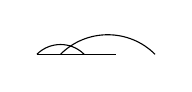
\begin{tikzpicture}
    \node (p) at (0, 0) {};
    \node (m) at (0.3, 0) {};
    \node (m2) at (0.6, 0) {};
    \node (q) at (1, 0) {};
    \node (o) at (1.5, 0) {};
    \draw (p.center) -- (q.center);
    \draw [out=45,in=135] (m.center) to (o.center);
    \draw [out=45,in=135] (p.center) to (m2.center);
  \end{tikzpicture} &
  \parbox{0.36\textwidth}{
    \textbf{$L$, Left}
    Same as $B$, but $o$--$(pq)$ edges may only be crossed by $p$--$(pq)$ edges. \\
  } \\
  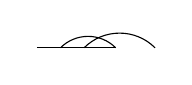
\begin{tikzpicture}
    \node (p) at (0, 0) {};
    \node (m) at (0.3, 0) {};
    \node (m2) at (0.6, 0) {};
    \node (q) at (1, 0) {};
    \node (o) at (1.5, 0) {};
    \draw (p.center) -- (q.center);
    \draw [out=45,in=135] (m2.center) to (o.center);
    \draw [out=45,in=135] (m.center) to (q.center);
  \end{tikzpicture} &
  \parbox{0.36\textwidth}{
    \textbf{$R$, Right}
    Same as $L$, but with edges crossed by $q$--$(pq)$ edges rather than $p$-$(pq)$ edges. \\
  } \\
  \begin{tikzpicture}
    \node (p) at (0, 0) {};
    \node (m) at (0.5, 0) {};
    \node (q) at (1, 0) {};
    \node (o) at (1.5, 0) {};
    \draw (p.center) -- (q.center);
    \draw [out=45,in=135] (m.center) to (o.center);
  \end{tikzpicture} &
  \parbox{0.36\textwidth}{
    \textbf{$N$, Neither}
    An interval and a point, with a least one $o$--$(pq)$ edge.
    $o$--$(pq)$ edges can only be crossed by $pq$, not other $[pq]$--$[pq]$ edges. \\
  }
\end{tabular}

Comparing these definitions with the items in \textcite{ec}, we have one entirely new type, the Exterval, and we have added the requirement that the later items have at least one crossing of the specified type.
These changes are necessary to avoid derivational ambiguity when a structure falls into multiple classes.
Enforcing these difference involves changes throughout the deduction rules.

\subsubsection{Example Derivation}

\begin{figure}
\centering

\tikzset{% 
  leftChild/.style={%
    ->,
    >=Stealth,
    shorten >=1pt,
    thin
  }
}

\tikzset{% 
  rightChild/.style={%
    <-,
    >=Stealth,
    shorten <=1pt,
    thin
  }
}

\tikzset{% 
  len1/.style={%
    out=30,
    in=150
  }
}

\tikzset{% 
  len2/.style={%
    out=32,
    in=148
  }
}

\tikzset{% 
  len3/.style={%
    out=34,
    in=146
  }
}

\tikzset{% 
  len4/.style={%
    out=34,
    in=146
  }
}
\tikzset{% 
  extPoint/.style={%
    fill=black,regular polygon, regular polygon sides=4,inner sep=0.75pt
  }
}
\tikzset{% 
  myGuide/.style={%
    densely dotted,
    thick,
    color=black!25
  }
}

\begin{tikzpicture}
  \pgfmathsetlength{\vertSmall}{7.5ex}
  \pgfmathsetlength{\vertBig}{10ex}
  \pgfmathsetlength{\vertBigger}{12ex}

  \coordinate (offset) at (0.1, 0);
  \coordinate (voffset0) at (0, 0);
  \coordinate (voffset1) at (0, 0.05);

  \node (v0) at (0, 0) {};
  \node (w0) at (0, 0) {};
  \node (w1) at (2, 0) {};
  \node (w2) at (4, 0) {};
  \node (w3) at (6, 0) {};
  \node (w4) at (8, 0) {};
  \node (w5) at (10, 0) {};
  \node (w6) at (12, 0) {};

  \node (vA) [below=\vertBig of v0] {};
  \node (v1) [above=\vertSmall of v0] {};
  \node (v2) [above=\vertSmall of v1] {};
  \node (v3) [above=\vertSmall of v2] {};
  \node (v4) [above=\vertSmall of v3] {};
  \node (v5) [above=\vertSmall of v4] {};
  \node (v6) [above=\vertSmall of v5] {};

  \draw [myGuide] (w0 |- vA) -- (w0 |- v6);
  \draw [myGuide] (w1 |- vA) -- (w1 |- v6);
  \draw [myGuide] (w2 |- vA) -- (w2 |- v6);
  \draw [myGuide] (w3 |- vA) -- (w3 |- v2);
  \draw [myGuide] (w4 |- vA) -- (w4 |- v4);
  \draw [myGuide] (w5 |- vA) -- (w5 |- v2);
  \draw [myGuide] (w6 |- vA) -- (w6 |- v6);

  \node (w0text) [below=\vertBig of w0] {\strut ROOT};
  \node (w1text) [below=\vertBig of w1] {\strut We};
  \node (w2text) [below=\vertBig of w2] {\strut like};
  \node (w3text) [below=\vertBig of w3] {\strut to};
  \node (w4text) [below=\vertBig of w4] {\strut run};
  \node (w5text) [below=\vertBig of w5] {\strut fast};
  \node (w6text) [below=\vertBig of w6] {\strut .};

  \draw [rightChild,len2] ($(w0 |- vA) + (offset)$) to ($(w2 |- vA) + (voffset1)$);
  \draw [leftChild,len1] ($(w1 |- vA) + (offset)$) to ($(w2 |- vA) - (offset) + (voffset0)$);
  \draw [leftChild,len1] ($(w3 |- vA) + (offset)$) to ($(w4 |- vA) - (offset) - (offset) + (voffset0)$);
  \draw [leftChild,len3] ($(w1 |- vA)$) to ($(w4 |- vA) + (voffset1)$);
  \draw [rightChild,len2] ($(w2 |- vA) + (offset) + (voffset0)$) to ($(w4 |- vA) - (offset)$);
  \draw [rightChild,len1] ($(w4 |- vA) + (offset) + (voffset0)$) to ($(w5 |- vA) - (offset)$);
  \draw [rightChild,len4] ($(w2 |- vA) + (voffset1)$) to ($(w6 |- vA) - (offset)$);

  \draw ($(w0) + (offset)$) -- node[at start,below=-2pt] {\small I} ($(w1) - (offset)$);
  \draw ($(w1) + (offset)$) -- node[at start,below=-2pt] {\small I} ($(w2) - (offset)$);
  \draw ($(w2) + (offset)$) -- node[at start,below=-2pt] {\small I} ($(w3) - (offset)$);
  \draw ($(w3) + (offset)$) -- node[at start,below=-2pt] {\small I} ($(w4) - (offset)$);
  \draw ($(w4) + (offset)$) -- node[at start,below=-2pt] {\small I} ($(w5) - (offset)$);
  \draw ($(w5) + (offset)$) -- node[at start,below=-2pt] {\small I} ($(w6) - (offset)$);
  \node [anchor=west] (step0) at (w6 |- v0) {\strut \small Initialize};

  \draw ($(w0 |- v1) + (offset)$) -- node[at start,below=-2pt] {\small X} ($(w1 |- v1) - (offset)$);
  \node [extPoint] at (w2 |- v1) {};
  \draw ($(w1 |- v1) + (offset)$) -- node[at start,below=-2pt] {\small I} ($(w2 |- v1) - (offset)$);
  \draw ($(w3 |- v1) + (offset)$) -- node[at start,below=-2pt] {\small I} ($(w4 |- v1) - (offset)$);
  \draw ($(w4 |- v1) + (offset)$) -- node[at start,below=-2pt] {\small I} ($(w5 |- v1) - (offset)$);
  \draw [rightChild,len2] ($(w0 |- v1) + (offset)$) to ($(w2 |- v1) + (voffset1)$);
  \draw [leftChild,len1] ($(w1 |- v1) + (offset)$) to ($(w2 |- v1) - (offset) + (voffset0)$);
  \draw [leftChild,len1] ($(w3 |- v1) + (offset)$) to ($(w4 |- v1) - (offset) + (voffset0)$);
  \draw [rightChild,len1] ($(w4 |- v1) + (offset) + (voffset0)$) to ($(w5 |- v1) - (offset)$);
  \node [anchor=west] (step0) at (w6 |- v1) {\strut \small Add edges};

  \draw ($(w2 |- v2) + (offset)$) -- node[at start,below=-2pt] {\small I} ($(w4 |- v2) - (offset)$);
  \draw ($(w4 |- v2) + (offset)$) -- node[at start,below=-2pt] {\small I} ($(w6 |- v2) - (offset)$);
  \draw [leftChild,len1] ($(w3 |- v2) + (offset)$) to ($(w4 |- v2) - (offset) + (voffset0)$);
  \draw [rightChild,len1] ($(w4 |- v2) + (offset) + (voffset0)$) to ($(w5 |- v2) - (offset)$);
  \node [anchor=west] (step0) at (w6 |- v2) {\strut \small Combine};

  \draw ($(w2 |- v3) + (offset)$) -- node[at start,below=-2pt] {\small X} ($(w4 |- v3) - (offset)$);
  \node [extPoint] at (w1 |- v3) {};
  \draw [leftChild,len1] ($(w3 |- v3) + (offset)$) to ($(w4 |- v3) - (offset) - (offset) + (voffset0)$);
  \draw [leftChild,len3] ($(w1 |- v3)$) to ($(w4 |- v3) + (voffset1)$);
  \draw [rightChild,len2] ($(w2 |- v3) + (offset) + (voffset0)$) to ($(w4 |- v3) - (offset)$);
  \node [anchor=west] (step0) at (w6 |- v3) {\strut \small Add edges};

  \draw ($(w2 |- v4) + (offset)$) -- node[at start,below=-2pt] {\small N} ($(w6 |- v4) - (offset)$);
  \node [extPoint] at (w1 |- v4) {};
  \draw [leftChild,len1] ($(w3 |- v4) + (offset)$) to ($(w4 |- v4) - (offset) - (offset) + (voffset0)$);
  \draw [leftChild,len3] ($(w1 |- v4)$) to ($(w4 |- v4) + (voffset1)$);
  \draw [rightChild,len2] ($(w2 |- v4) + (offset) + (voffset0)$) to ($(w4 |- v4) - (offset)$);
  \draw [rightChild,len1] ($(w4 |- v4) + (offset) + (voffset0)$) to ($(w5 |- v4) - (offset)$);
  \node [anchor=west] (step0) at (w6 |- v4) {\strut \small Combine};

  \draw ($(w2 |- v5) + (offset)$) -- node[at start,below=-2pt] {\small N} ($(w6 |- v5) - (offset)$);
  \node [extPoint] at (w1 |- v5) {};
  \draw [leftChild,len1] ($(w3 |- v5) + (offset)$) to ($(w4 |- v5) - (offset) - (offset) + (voffset0)$);
  \draw [leftChild,len3] ($(w1 |- v5)$) to ($(w4 |- v5) + (voffset1)$);
  \draw [rightChild,len2] ($(w2 |- v5) + (offset) + (voffset0)$) to ($(w4 |- v5) - (offset)$);
  \draw [rightChild,len1] ($(w4 |- v5) + (offset) + (voffset0)$) to ($(w5 |- v5) - (offset)$);
  \draw [rightChild,len4] ($(w2 |- v5) + (voffset1)$) to ($(w6 |- v5) - (offset)$);
  \node [anchor=west] (step0) at (w6 |- v5) {\strut \small Add edges};

  \draw ($(w0 |- v6) + (offset)$) -- node[at start,below=-2pt] {\small I} ($(w6 |- v6) - (offset)$);
  \draw [rightChild,len2] ($(w0 |- v6) + (offset)$) to ($(w2 |- v6) + (voffset1)$);
  \draw [leftChild,len1] ($(w1 |- v6) + (offset)$) to ($(w2 |- v6) - (offset) + (voffset0)$);
  \draw [leftChild,len1] ($(w3 |- v6) + (offset)$) to ($(w4 |- v6) - (offset) - (offset) + (voffset0)$);
  \draw [leftChild,len3] ($(w1 |- v6)$) to ($(w4 |- v6) + (voffset1)$);
  \draw [rightChild,len2] ($(w2 |- v6) + (offset) + (voffset0)$) to ($(w4 |- v6) - (offset)$);
  \draw [rightChild,len1] ($(w4 |- v6) + (offset) + (voffset0)$) to ($(w5 |- v6) - (offset)$);
  \draw [rightChild,len4] ($(w2 |- v6) + (voffset1)$) to ($(w6 |- v6) - (offset)$);
  \node [anchor=west] (step0) at (w6 |- v6) {\strut \small Combine};
\end{tikzpicture}

\vspace{-10mm}
\caption{\label{fig:alg-example}
An example derivation.
}
\end{figure}

Figure~\ref{fig:alg-example} presents a derivation of a sentence with crossing edges, showing examples of several deduction rules: \\
$\emptyset \mapsto I$ \hfill Initialization with intervals of span one \\
$I \land pq \mapsto I$ \hfill Adding the \emph{We}--\emph{like} edge\\
$I \land po \mapsto X$ \hfill Adding the \emph{like}--\emph{ROOT} edge \\
$I \land I \mapsto I$ \hfill Combining items either side of \emph{to} \\
$X \land I \mapsto N$ \hfill Combining items either side of \emph{run} \\
$X \land I \land N \mapsto I$ \hfill Final step

\subsubsection{Deduction Rules}
One set of deduction rules is concerned with removing direct edges between the points $p$, $q$, and $o$ in each item.
These are straightforward, so we leave them for the supplementary materials.

The other type of deduction rules, which we sketch below, involve decomposing an item into parts.
Since our item types are entirely disjoint, throughout the rules below we need to give multiple options for item types in many places where \textcite{ec} give only one type.

Here we describe the rules top-down, using properties of the complete item to determine how it is decomposed.
In this way we can show completeness, as we cover all possible settings of the properties we consider.

\paragraph{Interval}\label{sec:interval}
Is there a $p$--$(pq)$ edge? \\
No, then split at $p+1$: \\
\begin{tightflushright}
\begin{tikzpicture}
  \pgfmathsetlength{\vertSmall}{2ex}
  \pgfmathsetlength{\labelGap}{1ex}
  \pgfmathsetlength{\coordGap}{-0.5ex}
  \node (hlref) at (0, 0) {};
  \node (hmref) at (1, 0) {};
  \node (hrref) at (4, 0) {};

  \node (p0) at (hlref) {};
  \node (s0a) at (hmref) {};
  \node (v0bref) [below=\vertSmall of p0.center] {};
  \node (s0b) at (v0bref -| hmref) {};
  \node (q0) at (v0bref -| hrref) {};
  \node (label0) [left=\labelGap of p0] {$I$};
  \node (label0) [left=\labelGap of v0bref] {$I$};
  \draw (p0.center) -- (s0a.center);
  \draw (s0b.center) -- (q0.center);

  \node (lb) at (v0bref -| hlref) {};
  \node (sb) at (v0bref -| hmref) {};
  \node (rb) at (v0bref -| hrref) {};
  \node (ltext) [below=\coordGap of lb.center] {\small \strut $p$};
  \node (stext) [below=\coordGap of sb.center] {\small \strut ${p+1}$};
  \node (rtext) [below=\coordGap of rb.center] {\small \strut $q$};
\end{tikzpicture}
\end{tightflushright} \\
Yes, then consider $ps$, the longest $p$--$(pq)$ edge. \\
Do any edges cross $ps$? \\
No, then split at $s$: \\
\begin{tightflushright}
\begin{tikzpicture}
  \pgfmathsetlength{\vertSmall}{2ex}
  \pgfmathsetlength{\labelGap}{1ex}
  \pgfmathsetlength{\coordGap}{-0.5ex}
  \node (hlref) at (0, 0) {};
  \node (hmref) at (2, 0) {};
  \node (hrref) at (4, 0) {};

  \node (p0) at (hlref) {};
  \node (s0a) at (hmref) {};
  \node (v0bref) [below=\vertSmall of p0.center] {};
  \node (s0b) at (v0bref -| hmref) {};
  \node (q0) at (v0bref -| hrref) {};
  \node (label0) [left=\labelGap of p0] {$I$};
  \node (label0) [left=\labelGap of v0bref] {$I$};
  \draw (p0.center) -- (s0a.center);
  \draw (s0b.center) -- (q0.center);
  \draw [required,out=30,in=150] (p0.center) to (s0a.center);

  \node (lb) at (v0bref -| hlref) {};
  \node (sb) at (v0bref -| hmref) {};
  \node (rb) at (v0bref -| hrref) {};
  \node (ltext) [below=\coordGap of lb.center] {\small \strut $p$};
  \node (stext) [below=\coordGap of sb.center] {\small \strut $s$};
  \node (rtext) [below=\coordGap of rb.center] {\small \strut $q$};
\end{tikzpicture}
\end{tightflushright} \\
Yes, then consider the set of edges $C$, that cross $ps$.
If $|C| > 1$, let $t$ be the common endpoint of all edges in $C$ (they must have a common endpoint to satisfy the 1ec property for $ps$).
If $|C| = 1$, let $t$ be the endpoint outside $ps$ (this is one source of ambiguity in \textcite{ec}).

\noindent
Is $s < t$ and are there any $s$--$(tq)$ edges? \\
Yes to both: \\
\begin{tightflushright}
\begin{tikzpicture}
  \pgfmathsetlength{\vertSmall}{2ex}
  \pgfmathsetlength{\labelGap}{1ex}
  \pgfmathsetlength{\coordGap}{-0.5ex}
  \node (l) at (0, 0) {};
  \node (ls) at (0.5, 0) {};
  \node (s) at (1.5, 0) {};
  \node (t) at (2.5, 0) {};
  \node (tr) at (3.5, 0) {};
  \node (r) at (4, 0) {};

  \node (v0) at (l) {};
  \node (p0) at (v0 -| l) {};
  \node (q0) at (v0 -| s) {};
  \node (o0) at (v0 -| t) {};
  \node [pointO] at (o0) {};
  \node (label0) [left=\labelGap of v0] {$R$ or $N$};
  \node (v1) [below=\vertSmall of v0.center] {};
  \node (p1) at (v1 -| s) {};
  \node (q1) at (v1 -| t) {};
  \node (label1) [left=\labelGap of v1] {$I$};
  \node (v2) [below=\vertSmall of v1.center] {};
  \node (p2) at (v2 -| t) {};
  \node (q2) at (v2 -| r) {};
  \node (o2) at (v2 -| s) {};
  \node [pointO] at (o2) {};
  \node (label2) [left=\labelGap of v2] {$L$, $N$ or $X$};
  \draw (p0.center) -- (q0.center);
  \draw (p1.center) -- (q1.center);
  \draw (p2.center) -- (q2.center);
  \draw [required,out=30,in=150] (p0.center) to (q0.center);
  \draw [required,out=150,in=30] (o0.center) to (v0 -| ls);
  \draw [required,out=30,in=150] (o2.center) to (v2 -| tr);

  \node (lb) at (v2 -| l) {};
  \node (tb) at (v2 -| t) {};
  \node (sb) at (v2 -| s) {};
  \node (rb) at (v2 -| r) {};
  \node (ltext) [below=\coordGap of lb.center] {\small \strut $p$};
  \node (ttext) [below=\coordGap of tb.center] {\small \strut $t$};
  \node (stext) [below=\coordGap of sb.center] {\small \strut $s$};
  \node (rtext) [below=\coordGap of rb.center] {\small \strut $q$};
\end{tikzpicture}
\end{tightflushright} \\
Yes $s < t$, no $s$--$(tq)$ edges: \\
\begin{tightflushright}
\begin{tikzpicture}
  \pgfmathsetlength{\vertSmall}{2ex}
  \pgfmathsetlength{\labelGap}{1ex}
  \pgfmathsetlength{\coordGap}{-0.5ex}
  \node (l) at (0, 0) {};
  \node (ls) at (0.5, 0) {};
  \node (s) at (1.5, 0) {};
  \node (t) at (2.5, 0) {};
  \node (tr) at (3.5, 0) {};
  \node (r) at (4, 0) {};

  \node (v0) at (l) {};
  \node (p0) at (v0 -| l) {};
  \node (q0) at (v0 -| s) {};
  \node (o0) at (v0 -| t) {};
  \node [pointO] at (o0) {};
  \node (label0) [left=\labelGap of v0] {$B$, $L$, $R$ or $N$};
  \node (v1) [below=\vertSmall of v0.center] {};
  \node (p1) at (v1 -| s) {};
  \node (q1) at (v1 -| t) {};
  \node (label1) [left=\labelGap of v1] {$I$};
  \node (v2) [below=\vertSmall of v1.center] {};
  \node (p2) at (v2 -| t) {};
  \node (q2) at (v2 -| r) {};
  \node (label2) [left=\labelGap of v2] {$I$};
  \draw (p0.center) -- (q0.center);
  \draw (p1.center) -- (q1.center);
  \draw (p2.center) -- (q2.center);
  \draw [required,out=30,in=150] (p0.center) to (q0.center);
  \draw [required,out=150,in=30] (o0.center) to (v0 -| ls);

  \node (lb) at (v2 -| l) {};
  \node (tb) at (v2 -| t) {};
  \node (sb) at (v2 -| s) {};
  \node (rb) at (v2 -| r) {};
  \node (ltext) [below=\coordGap of lb.center] {\small \strut $p$};
  \node (ttext) [below=\coordGap of tb.center] {\small \strut $t$};
  \node (stext) [below=\coordGap of sb.center] {\small \strut $s$};
  \node (rtext) [below=\coordGap of rb.center] {\small \strut $q$};
\end{tikzpicture}
\end{tightflushright} \\
In this case it is also possible that $t = q$, in which case there is no $[tq]$ item.

\noindent
Now consider $s > t$.
In this case $C > 1$ by construction.
Are there any $p$--$(ts)$ edges? \\
Yes: \\
\begin{tightflushright}
\begin{tikzpicture}
  \pgfmathsetlength{\vertSmall}{2ex}
  \pgfmathsetlength{\labelGap}{1ex}
  \pgfmathsetlength{\coordGap}{-0.5ex}
  \node (l) at (0, 0) {};
  \node (t) at (1.5, 0) {};
  \node (ts) at (2, 0) {};
  \node (s) at (2.5, 0) {};
  \node (sr1) at (3, 0) {};
  \node (sr2) at (3.5, 0) {};
  \node (r) at (4, 0) {};

  \node (v0) at (l) {};
  \node (p0) at (v0 -| l) {};
  \node (q0) at (v0 -| t) {};
  \node (label0) [left=\labelGap of v0] {$I$};
  \node (v1) [below=\vertSmall of v0.center] {};
  \node (p1) at (v1 -| t) {};
  \node (q1) at (v1 -| s) {};
  \node (o1) at (v1 -| p) {};
  \node [pointO] at (o1) {};
  \node (label1) [left=\labelGap of v1] {$L$ or $N$};
  \node (v2) [below=\vertSmall of v1.center] {};
  \node (p2) at (v2 -| s) {};
  \node (q2) at (v2 -| r) {};
  \node (o2) at (v2 -| t) {};
  \node [pointO] at (o2) {};
  \node (label2) [left=\labelGap of v2] {$N$};
  \draw (p0.center) -- (q0.center);
  \draw (p1.center) -- (q1.center);
  \draw (p2.center) -- (q2.center);
  \draw [required,out=30,in=150] (o1.center) to (q1.center);
  \draw [required,out=30,in=150] (o1.center) to (v1 -| ts);
  \draw [required,out=30,in=150] (o2.center) to (v2 -| sr1);
  \draw [required,out=30,in=150] (o2.center) to (v2 -| sr2);

  \node (lb) at (v2 -| l) {};
  \node (tb) at (v2 -| t) {};
  \node (sb) at (v2 -| s) {};
  \node (rb) at (v2 -| r) {};
  \node (ltext) [below=\coordGap of lb.center] {\small \strut $p$};
  \node (ttext) [below=\coordGap of tb.center] {\small \strut $t$};
  \node (stext) [below=\coordGap of sb.center] {\small \strut $s$};
  \node (rtext) [below=\coordGap of rb.center] {\small \strut $q$};
\end{tikzpicture}
\end{tightflushright} \\
No: \\
\begin{tightflushright}
\begin{tikzpicture}
  \pgfmathsetlength{\vertSmall}{2ex}
  \pgfmathsetlength{\labelGap}{1ex}
  \pgfmathsetlength{\coordGap}{-0.5ex}
  \node (l) at (0, 0) {};
  \node (t) at (1.5, 0) {};
  \node (ts) at (2, 0) {};
  \node (s) at (2.5, 0) {};
  \node (sr1) at (3, 0) {};
  \node (sr2) at (3.5, 0) {};
  \node (r) at (4, 0) {};

  \node (v0) at (l) {};
  \node (p0) at (v0 -| l) {};
  \node (q0) at (v0 -| t) {};
  \node (o0) at (v0 -| s) {};
  \node [pointO] at (o0) {};
  \node (label0) [left=\labelGap of v0] {$R$, $N$ or $X$};
  \node (v1) [below=\vertSmall of v0.center] {};
  \node (p1) at (v1 -| t) {};
  \node (q1) at (v1 -| s) {};
  \node (label1) [left=\labelGap of v1] {$I$};
  \node (v2) [below=\vertSmall of v1.center] {};
  \node (p2) at (v2 -| s) {};
  \node (q2) at (v2 -| r) {};
  \node (o2) at (v2 -| t) {};
  \node [pointO] at (o2) {};
  \node (label2) [left=\labelGap of v2] {$N$};
  \draw (p0.center) -- (q0.center);
  \draw (p1.center) -- (q1.center);
  \draw (p2.center) -- (q2.center);
  \draw [required,out=30,in=150] (p0.center) to (o0.center);
  \draw [required,out=30,in=150] (o2.center) to (v2 -| sr1);
  \draw [required,out=30,in=150] (o2.center) to (v2 -| sr2);

  \node (lb) at (v2 -| l) {};
  \node (tb) at (v2 -| t) {};
  \node (sb) at (v2 -| s) {};
  \node (rb) at (v2 -| r) {};
  \node (ltext) [below=\coordGap of lb.center] {\small \strut $p$};
  \node (ttext) [below=\coordGap of tb.center] {\small \strut $t$};
  \node (stext) [below=\coordGap of sb.center] {\small \strut $s$};
  \node (rtext) [below=\coordGap of rb.center] {\small \strut $q$};
\end{tikzpicture}
\end{tightflushright}

\paragraph{Exterval}
No decomposition rules are needed, as the removal of the $op$ or $oq$ edge leaves behind an Interval.

\paragraph{Both} \label{sec:alg:both}
Consider the case when $o$ is to the right (the case when $o$ is to the left is symmetrical).
Consider $ps_p$, the longest $p$--$(pq)$ edge. \\
Does $ps_p$ cross any $q$--$(pq)$ edges? \\
Yes: \\
\begin{tightflushright}
\begin{tikzpicture}
  \pgfmathsetlength{\vertSmall}{2ex}
  \pgfmathsetlength{\labelGap}{1ex}
  \pgfmathsetlength{\coordGap}{-0.5ex}
  \node (l) at (0, 0) {};
  \node (t) at (1.5, 0) {};
  \node (ts) at (2, 0) {};
  \node (s) at (2.5, 0) {};
  \node (sr1) at (3, 0) {};
  \node (sr2) at (3.5, 0) {};
  \node (r) at (4, 0) {};
  \node (o) at (5, 0) {};

  \node (v0) at (l) {};
  \node (p0) at (v0 -| l) {};
  \node (q0) at (v0 -| t) {};
  \node (o0) at (v0 -| s) {};
  \node [pointO] at (o0) {};
  \node (label0) [left=\labelGap of v0] {$R$, $N$ or $X$};
  \node (v1) [below=\vertSmall of v0.center] {};
  \node (p1) at (v1 -| t) {};
  \node (q1) at (v1 -| s) {};
  \node (o1) at (v1 -| o) {};
  \node [pointO] at (o1) {};
  \node (label1) [left=\labelGap of v1] {$X'$};
  \node (v2) [below=\vertSmall of v1.center] {};
  \node (p2) at (v2 -| s) {};
  \node (q2) at (v2 -| r) {};
  \node (o2) at (v2 -| t) {};
  \node [pointO] at (o2) {};
  \node (label2) [left=\labelGap of v2] {$L$, $N$ or $X$};
  \draw (p0.center) -- (q0.center);
  \draw (p1.center) -- (q1.center);
  \draw (p2.center) -- (q2.center);
  \draw [required,out=30,in=150] (p0.center) to (o0.center);
  \draw [required,out=30,in=150] (o2.center) to (q2.center);
  \draw [required,out=20,in=160] (p1.center) to (o1.center);
  \draw [required,out=20,in=160] (q1.center) to (o1.center);

  \node (lb) at (v2 -| l) {};
  \node (tb) at (v2 -| t) {};
  \node (sb) at (v2 -| s) {};
  \node (rb) at (v2 -| r) {};
  \node (ob) at (v2 -| o) {};
  \node (ltext) [below=\coordGap of lb.center] {\small \strut $p$};
  \node (ttext) [below=\coordGap of tb.center] {\small \strut $s_p$};
  \node (stext) [below=\coordGap of sb.center] {\small \strut $s_q$};
  \node (rtext) [below=\coordGap of rb.center] {\small \strut $q$};
  \node (otext) [below=\coordGap of ob.center] {\small \strut $o$};
\end{tikzpicture}
\end{tightflushright}

The extra edges shown must be present because of the definition of $B$ items and the 1ec property.
The $X'$ is a slight variation on our $X$, since it has both $s_qo$ and $s_po$.
This structure does not come up in \textcite{ec}'s algorithm because of tree constraints that apply once directionality is considered.
We do not include this rule because it would be $O(n^5)$, and this specific structure is almost never observed in the treebank.

Now consider the alternative, when $ps_p$ does not cross any $q$--$(pq)$ edges.
In this case the possibilities follow a pattern: \\\vspace{-2mm}
\begin{center}
\begin{tikzpicture}
  \node (p) at (1, 0) {};
  \node (m0) at (1.5, 0) {};
  \node (sp) at (2, 0) {};
  \node (sq) at (4, 0) {};
  \node (m1) at (4.5, 0) {};
  \node (q) at (5, 0) {};
  \node (o) at (6, 0) {};
  \node [pointO] at (o.north) {};
  \draw (p.north) -- (q.north);
  \draw [out=45,in=135] (p.north) to (sp.north);
  \draw [out=45,in=135] (sq.north) to (q.north);
  \draw [out=20,in=160] (m0.north) to (o.north);
  \draw [out=20,in=160] (m1.north) to (o.north);
\end{tikzpicture} \\\vspace{-2mm}
\begin{tikzpicture}
  \node (p) at (1, 0) {};
  \node (m0) at (1.5, 0) {};
  \node (sp) at (2, 0) {};
  \node (m2) at (2.5, 0) {};
  \node (sq) at (4, 0) {};
  \node (m1) at (4.5, 0) {};
  \node (q) at (5, 0) {};
  \node (o) at (6, 0) {};
  \node [pointO] at (o.north) {};
  \draw (p.north) -- (q.north);
  \draw [out=45,in=135] (p.north) to (sp.north);
  \draw [out=45,in=135] (sq.north) to (q.north);
  \draw [out=25,in=155] (m0.north) to (m2.north);
  \draw [out=20,in=160] (m0.north) to (o.north);
  \draw [out=20,in=160] (m1.north) to (o.north);
\end{tikzpicture} \\\vspace{-2mm}
\begin{tikzpicture}
  \node (p) at (1, 0) {};
  \node (m0) at (1.5, 0) {};
  \node (s) at (2, 0) {};
  \node (m2) at (2.5, 0) {};
  \node (m3) at (3, 0) {};
  \node (sq) at (4, 0) {};
  \node (m1) at (4.5, 0) {};
  \node (q) at (5, 0) {};
  \node (o) at (6, 0) {};
  \node [pointO] at (o.north) {};
  \draw (p.north) -- (q.north);
  \draw [out=45,in=135] (p.north) to (s.north);
  \draw [out=45,in=135] (sq.north) to (q.north);
  \draw [out=25,in=155] (m0.north) to (m2.north);
  \draw [out=20,in=160] (m0.north) to (o.north);
  \draw [out=20,in=160] (m1.north) to (o.north);
  \draw [out=25,in=155] (s.north) to (m3.north);
\end{tikzpicture} \\\vspace{-2mm}
\begin{tikzpicture}
  \node (p) at (1, 0) {};
  \node (m0) at (1.5, 0) {};
  \node (s) at (2, 0) {};
  \node (m2) at (2.5, 0) {};
  \node (m3) at (3, 0) {};
  \node (m4) at (3.5, 0) {};
  \node (sq) at (4, 0) {};
  \node (m1) at (4.5, 0) {};
  \node (q) at (5, 0) {};
  \node (o) at (6, 0) {};
  \node [pointO] at (o.north) {};
  \draw (p.north) -- (q.north);
  \draw [out=45,in=135] (p.north) to (s.north);
  \draw [out=45,in=135] (sq.north) to (q.north);
  \draw [out=25,in=155] (m0.north) to (m2.north);
  \draw [out=20,in=160] (m0.north) to (o.north);
  \draw [out=20,in=160] (m1.north) to (o.north);
  \draw [out=25,in=155] (s.north) to (m3.north);
  \draw [out=25,in=155] (m2.north) to (m4.north);
\end{tikzpicture} \\\vspace{-2mm}
\begin{tikzpicture}
  \node (p) at (1, 0) {};
  \node (m0) at (1.5, 0) {};
  \node (s) at (2, 0) {};
  \node (m2) at (2.5, 0) {};
  \node (m3) at (3, 0) {};
  \node (m4) at (3.5, 0) {};
  \node (sq) at (4, 0) {};
  \node (m1) at (4.5, 0) {};
  \node (q) at (5, 0) {};
  \node (o) at (6, 0) {};
  \node [pointO] at (o.north) {};
  \draw [out=45,in=135] (p.north) to (s.north);
  \draw [out=45,in=135] (sq.north) to (q.north);
  \draw [out=25,in=155] (m0.north) to (m2.north);
  \draw [out=20,in=160] (m0.north) to (o.north);
  \draw [out=20,in=160] (m1.north) to (o.north);
  \draw [out=25,in=155] (s.north) to (m3.north);
  \draw [out=25,in=155] (m2.north) to (m4.north);
  \draw [out=25,in=155] (m4.north) to (m1.north);
  \draw [out=25,in=155] (m3.north) to (sq.north);
  \node [fill=white] (dots) at (3,0.25) {\small . . .};
  \draw (p.north) -- (q.north);
\end{tikzpicture}
\end{center}

Does the pattern go all the way to the right, as shown in the last case? \\
Yes: \\
\begin{tightflushright}
\parbox{0.42\textwidth}{
We cannot define a simple decomposition of the structure using our item types.
By eliminating this case we restrict ourselves to a subset of one-endpoint-crossing graphs.
This does not decrease treebank coverage. \\
}
\end{tightflushright}

\noindent
No, then use the end of the edge crossing pattern as $s$ and decompose the item as: \\
\begin{tightflushright}
\begin{tikzpicture}
  \pgfmathsetlength{\vertSmall}{2ex}
  \pgfmathsetlength{\labelGap}{1ex}
  \pgfmathsetlength{\coordGap}{-0.5ex}
  \node (l) at (0, 0) {};
  \node (ls) at (1, 0) {};
  \node (s) at (2, 0) {};
  \node (sr) at (3, 0) {};
  \node (r) at (4, 0) {};
  \node (o) at (5, 0) {};

  \node (v0) at (l) {};
  \node (p0) at (v0 -| l) {};
  \node (q0) at (v0 -| s) {};
  \node (o0) at (v0 -| o) {};
  \node [pointO] at (o0) {};
  \node (label0) [left=\labelGap of v0] {$L$ or $N$};
  \node (v1) [below=\vertSmall of v0.center] {};
  \node (p1) at (v1 -| s) {};
  \node (q1) at (v1 -| r) {};
  \node (o1) at (v1 -| o) {};
  \node [pointO] at (o1) {};
  \node (label1) [left=\labelGap of v1] {$R$ or $N$};
  \draw (p0.center) -- (q0.center);
  \draw (p1.center) -- (q1.center);
  \draw [optional,out=30,in=150] (p0.center) to (q0.center);
  \draw [optional,out=30,in=150] (p1.center) to (q1.center);
  \draw [required,out=20,in=160] (v0 -| ls) to (o0.center);
  \draw [required,out=30,in=150] (v1 -| sr) to (o1.center);

  \node (lb) at (v1 -| l) {};
  \node (sb) at (v1 -| s) {};
  \node (rb) at (v1 -| r) {};
  \node (ob) at (v1 -| o) {};
  \node (ltext) [below=\coordGap of lb.center] {\small \strut $p$};
  \node (stext) [below=\coordGap of sb.center] {\small \strut $s$};
  \node (rtext) [below=\coordGap of rb.center] {\small \strut $q$};
  \node (otext) [below=\coordGap of ob.center] {\small \strut $o$};
\end{tikzpicture}
\end{tightflushright}

The dashed edges are required for the $N$ items, but not the $L$ items.
The choice of split point in this case is one source of derivational ambiguity in \textcite{ec}.
Below we describe how to check that the chaining pattern is present in an $L$, but in practice we avoid it entirely by requiring the $L$ to have the edge $ps$, with no loss in coverage.

\paragraph{Left and Right}
These are defined symmetrically.
Consider the $o$--$(pq)$ edges in an $L$.
Use the edge $os$ with $s$ furthest from $p$ to define the split point.

\noindent
Is $os$ crossed by any $p$--$(pq)$ edges? \\
No: \\
\begin{tightflushright}
\begin{tikzpicture}
  \pgfmathsetlength{\vertSmall}{2ex}
  \pgfmathsetlength{\labelGap}{1ex}
  \pgfmathsetlength{\coordGap}{-0.5ex}
  \node (l) at (0, 0) {};
  \node (ls) at (1, 0) {};
  \node (s) at (2, 0) {};
  \node (sr) at (3, 0) {};
  \node (r) at (4, 0) {};
  \node (o) at (5, 0) {};

  \node (v0) at (l) {};
  \node (p0) at (v0 -| l) {};
  \node (q0) at (v0 -| s) {};
  \node (o0) at (v0 -| o) {};
  \node [pointO] at (o0) {};
  \node (label0) [left=\labelGap of v0] {$L$ or $N$};
  \node (v1) [below=\vertSmall of v0.center] {};
  \node (p1) at (v1 -| s) {};
  \node (q1) at (v1 -| r) {};
  \node (label1) [left=\labelGap of v1] {$I$};
  \draw (p0.center) -- (q0.center);
  \draw (p1.center) -- (q1.center);
  \draw [required,out=20,in=160] (q0.center) to (o0.center);
  \draw [required,out=160,in=20] (o0.center) to (v0 -| ls);

  \node (lb) at (v1 -| l) {};
  \node (sb) at (v1 -| s) {};
  \node (rb) at (v1 -| r) {};
  \node (ob) at (v1 -| o) {};
  \node (ltext) [below=\coordGap of lb.center] {\small \strut $p$};
  \node (stext) [below=\coordGap of sb.center] {\small \strut $s$};
  \node (rtext) [below=\coordGap of rb.center] {\small \strut $q$};
  \node (otext) [below=\coordGap of ob.center] {\small \strut $o$};
\end{tikzpicture}
\end{tightflushright} \\
Yes, then is $os$ the only $o$--$(pq)$ edge? \\
Yes: \\
\begin{tightflushright}
\begin{tikzpicture}
  \pgfmathsetlength{\vertSmall}{2ex}
  \pgfmathsetlength{\labelGap}{1ex}
  \pgfmathsetlength{\coordGap}{-0.5ex}
  \node (l) at (0, 0) {};
  \node (ls) at (1, 0) {};
  \node (s) at (2, 0) {};
  \node (sr) at (3, 0) {};
  \node (r) at (4, 0) {};
  \node (o) at (5, 0) {};

  \node (v0) at (l) {};
  \node (p0) at (v0 -| l) {};
  \node (q0) at (v0 -| s) {};
  \node (o0) at (v0 -| o) {};
  \node [pointO] at (o0) {};
  \node (label0) [left=\labelGap of v0] {$X$};
  \node (v1) [below=\vertSmall of v0.center] {};
  \node (p1) at (v1 -| s) {};
  \node (q1) at (v1 -| r) {};
  \node (o1) at (v1 -| l) {};
  \node [pointO] at (o1) {};
  \node (label1) [left=\labelGap of v1] {$L$ or $N$};
  \draw (p0.center) -- (q0.center);
  \draw (p1.center) -- (q1.center);
  \draw [required,out=20,in=160] (q0.center) to (o0.center);
  \draw [required,out=20,in=160] (o1.center) to (v1 -| sr);

  \node (lb) at (v1 -| l) {};
  \node (sb) at (v1 -| s) {};
  \node (rb) at (v1 -| r) {};
  \node (ob) at (v1 -| o) {};
  \node (ltext) [below=\coordGap of lb.center] {\small \strut $p$};
  \node (stext) [below=\coordGap of sb.center] {\small \strut $s$};
  \node (rtext) [below=\coordGap of rb.center] {\small \strut $q$};
  \node (otext) [below=\coordGap of ob.center] {\small \strut $o$};
\end{tikzpicture}
\end{tightflushright} \\
No: \\
\begin{tightflushright}
\begin{tikzpicture}
  \pgfmathsetlength{\vertSmall}{2ex}
  \pgfmathsetlength{\labelGap}{1ex}
  \pgfmathsetlength{\coordGap}{-0.5ex}
  \node (l) at (0, 0) {};
  \node (ls) at (1, 0) {};
  \node (s) at (2, 0) {};
  \node (sr) at (3, 0) {};
  \node (r) at (4, 0) {};
  \node (o) at (5, 0) {};

  \node (v0) at (l) {};
  \node (p0) at (v0 -| l) {};
  \node (q0) at (v0 -| s) {};
  \node (o0) at (v0 -| o) {};
  \node [pointO] at (o0) {};
  \node (label0) [left=\labelGap of v0] {$L$ or $N$};
  \node (v1) [below=\vertSmall of v0.center] {};
  \node (p1) at (v1 -| s) {};
  \node (q1) at (v1 -| r) {};
  \node (o1) at (v1 -| l) {};
  \node [pointO] at (o1) {};
  \node (label1) [left=\labelGap of v1] {$N$};
  \draw (p0.center) -- (q0.center);
  \draw (p1.center) -- (q1.center);
  \draw [required,out=20,in=160] (q0.center) to (o0.center);
  \draw [required,out=20,in=160] (v0 -| ls) to (o0.center);
  \draw [required,out=20,in=160] (o1.center) to (v1 -| sr);

  \node (lb) at (v1 -| l) {};
  \node (sb) at (v1 -| s) {};
  \node (rb) at (v1 -| r) {};
  \node (ob) at (v1 -| o) {};
  \node (ltext) [below=\coordGap of lb.center] {\small \strut $p$};
  \node (stext) [below=\coordGap of sb.center] {\small \strut $s$};
  \node (rtext) [below=\coordGap of rb.center] {\small \strut $q$};
  \node (otext) [below=\coordGap of ob.center] {\small \strut $o$};
\end{tikzpicture}
\end{tightflushright}

Our decomposition of this item differs from \textcite{ec}'s in several ways because of our decision to separate edge creation and item combination.
We also have to track whether there are multiple edges or only a single $o$--$(pq)$ edge, to avoid derivational ambiguity in the $I$ decomposition.
The top and bottom cases lead to multiple such edges, while the middle case will only have one.
Finally, we could track the chaining property discussed in the previous section.
The property is only true in the following cases: when the edge $pq$ is present, when an $X$ is combined with an $L$ that has the property, and when an $X$ is combined with an $N$ that has the $pq$ edge.

\paragraph{Neither}
Consider the $o$--$(pq)$ edges.
Use the edge $os$ with $s$ furthest from $o$ to define the split point.
Is $o$ to the right of the span? \\
Yes: \\
\begin{tightflushright}
\begin{tikzpicture}
  \pgfmathsetlength{\vertSmall}{2ex}
  \pgfmathsetlength{\labelGap}{1ex}
  \pgfmathsetlength{\coordGap}{-0.5ex}
  \node (l) at (0, 0) {};
  \node (ls) at (1, 0) {};
  \node (s) at (2, 0) {};
  \node (sr) at (3, 0) {};
  \node (r) at (4, 0) {};
  \node (o) at (5, 0) {};

  \node (v0) at (l) {};
  \node (p0) at (v0 -| l) {};
  \node (q0) at (v0 -| s) {};
  \node (label0) [left=\labelGap of v0] {$I$};
  \node (v1) [below=\vertSmall of v0.center] {};
  \node (p1) at (v1 -| s) {};
  \node (q1) at (v1 -| r) {};
  \node (o1) at (v1 -| o) {};
  \node [pointO] at (o1) {};
  \node (label1) [left=\labelGap of v1] {$N$ or $X$};
  \draw (p0.center) -- (q0.center);
  \draw (p1.center) -- (q1.center);
  \draw [required,out=20,in=160] (p1.center) to (o1.center);

  \node (lb) at (v1 -| l) {};
  \node (sb) at (v1 -| s) {};
  \node (rb) at (v1 -| r) {};
  \node (ob) at (v1 -| o) {};
  \node (ltext) [below=\coordGap of lb.center] {\small \strut $p$};
  \node (stext) [below=\coordGap of sb.center] {\small \strut $s$};
  \node (rtext) [below=\coordGap of rb.center] {\small \strut $q$};
  \node (otext) [below=\coordGap of ob.center] {\small \strut $o$};
\end{tikzpicture}
\end{tightflushright} \\
No, symmetrical to the yes case.

As in the previous section, our decomposition differs from \textcite{ec}'s to meet our altered definition of $N$.
Here, when a sub-item is an $X$ there is only one $o$--$(pq)$ edge, and when it is an $N$ there is more than one.

\subsubsection{Extensions}
To handle our representation, we extend the core algorithm described above to support labels on edges and labels on words (spines).
Additionally, we can constrain the search space to structures containing a projective tree of non-trace edges.

\paragraph{Edge Labels and Spines}\label{sec:labels}
Edge labels can be added by calculating either the sum or max over edge types when adding each edge, and recording the chosen edge in the back reference for the state.
Spines must be added to the state definition, specifying a label for each visible word ($p$, $q$ and $o$).
This state expansion is necessary to ensure agreement when combining items.
\textcite{cck}'s projective tree parser uses a similar approach, while \textcite{ec}'s algorithm is for dependency parsing and so does not consider spines.

\paragraph{Enforcing a tree backbone}
The algorithm above constrains the space of graph structures, but we also want to restrict our search to parses containing a directed projective tree of non-trace edges.
This requirement is satisfied if every word is the child of exactly one non-trace edge, and no non-trace edges cross.

To meet the first condition we add booleans to the state, indicating whether $p$, $q$ and $o$ have non-trace parents.
When adding edges, a non-trace edge cannot be added if the child already has a non-trace parent.
When combining items, no word can receive multiple non-trace parents, and words in the middle of the span must have at least one.

Crossing edges are introduced in two ways:
(1) when adding a $pq$ edge in the $N$, $L$, $R$ and $B$ items, and
(2) when a non-$B$ item is being formed using two non-$I$ items.
In both cases we can avoid non-trace edges crossing by using a boolean that tracks whether there are non-trace $o$--$[pq]$ edges in each item.
The justification is complex and can be found in the supplementary material.

\subsubsection{Derivational ambiguity}

One key difference between our algorithm and the original one-endpoint-crossing algorithm presented by \textcite{ec} is that we avoid spurious ambiguity in the ways a parse can be decomposed.
Most of the cases in which this ambiguity arises are due to symmetry that is not explicitly broken.
For example, the choice of $t$ in the description of Intervals.
We resolved these issues by breaking such cases of symmetry, and altering the definitions of the items to ensure they cannot represent equivalent structures.
By avoiding derivational ambiguity we reduce the search space, and enable efficient summing over the space.

\subsubsection{Complexity}

Without any labels, our algorithm is $O(n^4)$, where $n$ is the length of the sentence.
This comes from both the ternary deduction rules, which require two endpoints and two split points, and many of the binary deduction rules, which have two endpoints, a split point, and an external point.

Adding edge labels changes the complexity to $O(n^4 + e n^2)$, where $e$ is the number of edge types, and the second term comes from having to score every possible edge.
Adding spines, changes the complexity to $O(s^4 n^4 + e s^2 n^2)$, where $s$ is the number of spine types, though depending on features the second term could be simplified to either $e n^2$ or $s^2 n^2$.
In constituency parsing $e$ and $s$ are both around a thousand, making full enumeration of the dynamic program too slow in practice.
We resolve this issue through several types of pruning, described in the next section.

Finally, there is an important constant in the complexity, relating to the number of rules.
For any set of split points there are multiple items that could be combined.
Once our templates are expanded to show the possible state combinations there are 49,292 rules.

%%%\subsubsection{Inside-Outside}

%%%When using our algorithm with a model that only places weights on the edges, computing max-marginals and sum-marginals is straightforward.
%%%Each edge exists in only one place in the derivation, between the item without it and the item with it.

%%%Once spines are introduced the situation changes because we would like to score them in all of the items they appear in.
%%%This scoring is important for



\subsection{Complete Dynamic Program}

\begin{figure*}
\begin{multicols}{3}
\scalebox{\mathscale}{\parbox{\linewidth}{
\begin{flalign*}
& \begin{array}{l}
  \uwave{L}[ijx \; .\overline{X} \; .X \; \overline{IJ}] \leftarrow \max \\
  \;\;\; A[x \; j] \quad L[ijx \; .\overline{X} \; .\overline{X} \; \overline{IJ}] \\
\end{array} \\
& \begin{array}{l}
  \uwave{L}[ijx \; .\overline{X} \; .\overline{X} \; \overline{I}J] \leftarrow \max \\
  \;\;\; A[j \; x] \quad L[ijx \; .\overline{X} \; .\overline{X} \; \overline{IJ}] \\
\end{array} \\
& \begin{array}{l}
  L[ijx \; J\overline{X} \; \overline{IX} \; \overline{IJ}] \leftarrow \max \\
  \;\;\; A[j \; i] \quad L[ijx \; \overline{JX} \; \overline{IX} \; \overline{IJ}] \\
\end{array} \\
& \begin{array}{l}
  L[ijx \; \overline{JX} \; I\overline{X} \; \overline{IJ}] \leftarrow \max \\
  \;\;\; A[i \; j] \quad L[ijx \; \overline{JX} \; \overline{IX} \; \overline{IJ}] \\
\end{array} \\
& \begin{array}{l}
  \uwave{R}[ijx \; .X \; .\overline{X} \; \overline{IJ}] \leftarrow \max \\
  \;\;\; A[x \; i] \quad R[ijx \; .\overline{X} \; .\overline{X} \; \overline{IJ}] \\
\end{array} \\
& \begin{array}{l}
  \uwave{R}[ijx \; .\overline{X} \; .\overline{X} \; I\overline{J}] \leftarrow \max \\
  \;\;\; A[i \; x] \quad R[ijx \; .\overline{X} \; .\overline{X} \; \overline{IJ}] \\
\end{array} \\
& \begin{array}{l}
  R[ijx \; J\overline{X} \; \overline{IX} \; \overline{IJ}] \leftarrow \max \\
  \;\;\; A[j \; i] \quad R[ijx \; \overline{JX} \; \overline{IX} \; \overline{IJ}] \\
\end{array} \\
& \begin{array}{l}
  R[ijx \; \overline{JX} \; I\overline{X} \; \overline{IJ}] \leftarrow \max \\
  \;\;\; A[i \; j] \quad R[ijx \; \overline{JX} \; \overline{IX} \; \overline{IJ}] \\
\end{array}
\end{flalign*}
}}

\scalebox{\mathscale}{\parbox{\linewidth}{
\begin{flalign*}
& \begin{array}{l}
  \uwave{N}[ijx \; .X \; .\overline{X} \; \overline{IJ}] \leftarrow \max \\
  \;\;\; A[x \; i] \quad N[ijx \; .\overline{X} \; .\overline{X} \; \overline{IJ}] \\
\end{array} \\
& \begin{array}{l}
  \uwave{N}[ijx \; .\overline{X} \; .\overline{X} \; I\overline{J}] \leftarrow \max \\
  \;\;\; A[i \; x] \quad N[ijx \; .\overline{X} \; .\overline{X} \; \overline{IJ}] \\
\end{array} \\
& \begin{array}{l}
  \uwave{N}[ijx \; .\overline{X} \; .X \; \overline{IJ}] \leftarrow \max \\
  \;\;\; A[x \; j] \quad N[ijx \; .\overline{X} \; .\overline{X} \; \overline{IJ}] \\
\end{array} \\
& \begin{array}{l}
  \uwave{N}[ijx \; .\overline{X} \; .\overline{X} \; \overline{I}J] \leftarrow \max \\
  \;\;\; A[j \; x] \quad N[ijx \; .\overline{X} \; .\overline{X} \; \overline{IJ}] \\
\end{array} \\
& \begin{array}{l}
  N[ijx \; J\overline{X} \; \overline{IX} \; \overline{IJ}] \leftarrow \max \\
  \;\;\; A[j \; i] \quad N[ijx \; \overline{JX} \; \overline{IX} \; \overline{IJ}] \\
\end{array} \\
& \begin{array}{l}
  N[ijx \; \overline{JX} \; I\overline{X} \; \overline{IJ}] \leftarrow \max \\
  \;\;\; A[i \; j] \quad N[ijx \; \overline{JX} \; \overline{IX} \; \overline{IJ}] \\
\end{array} \\
& \begin{array}{l}
  B\cdotp [ijx \; F \; I\overline{X} \; \overline{IJ}] \leftarrow \max \\
  \;\;\; A[i \; j] \quad B\cdotp [ijx \; F \; \overline{IX} \; \overline{IJ}] \\
\end{array} \\
& \begin{array}{l}
  \cdotp B[ijx \; J\overline{X} \; F \; \overline{IJ}] \leftarrow \max \\
  \;\;\; A[j \; i] \quad \cdotp B[ijx \; \overline{JX} \; F \; \overline{IJ}] \\
\end{array}
\end{flalign*}
}}

\scalebox{\mathscale}{\parbox{\linewidth}{
\begin{flalign*}
& \begin{array}{l}
  I[ij \; F \; I] \leftarrow \max \\
  \;\;\; A[i \; j] \quad I[ij \; F \; \overline{I}] \\
\end{array} \\
& \begin{array}{l}
  I[ij \; J \; F] \leftarrow \max \\
  \;\;\; A[j \; i] \quad I[ij \; \overline{J} \; F] \\
\end{array} \\
\\
\\
\\
& \begin{array}{l}
  X[ijx \; .X \; .\overline{X} \; F] \leftarrow \max \\
  \;\;\; A[x \; i] \quad I[ij \; . \; .] \\
\end{array} \\
& \begin{array}{l}
  X[ijx \; .\overline{X} \; .\overline{X} \; I\overline{J}] \leftarrow \max \\
  \;\;\; A[i \; x] \quad I[ij \; . \; .] \\
\end{array} \\
& \begin{array}{l}
  X[ijx \; .\overline{X} \; .X \; F] \leftarrow \max \\
  \;\;\; A[x \; j] \quad I[ij \; . \; .] \\
\end{array} \\
& \begin{array}{l}
  X[ijx \; .\overline{X} \; .\overline{X} \; \overline{I}J] \leftarrow \max \\
  \;\;\; A[j \; x] \quad I[ij \; . \; .] \\
\end{array}
\end{flalign*}
}}
\end{multicols}

\vspace{-10mm}
\begin{multicols}{2}
\scalebox{\mathscale}{\parbox{\linewidth}{
\begin{flalign*}
& \begin{array}{l}
  I[ij \; F \; \overline{I}] \leftarrow \max \\
\end{array} \\
& \left\{
  \begin{array}{l}
    \begin{array}{l}
      I[i \; i{+}1 \; F \; F] \quad I[i{+}1 \; j \; \overline{F} \; F] \\
    \end{array} \\
    \max_{k \in (i, j)} \\
    \left\{
      \begin{array}{l}
        I[ik \; F \; I] \quad I[kj \; . \; .] \\
        BLRN\cdotp [ikj \; F \; I\overline{J} \; \overline{IK}] \quad I[kj \; . \; .] \\
        \max_{l \in (k, j)} \\
        \left\{
          \begin{array}{l}
            RN\cdotp [ikl \; F \; I\overline{L} \; \overline{IK}] \quad I[kl \; . \; .] \quad \cdotp LNX[ljk \; .\overline{K} \; . \; \overline{L}.] \\
            BLRN\cdotp [ikl \; F \; I\overline{L} \; \overline{IK}] \quad I[kl \; . \; .] \quad I[lj \; . \; .] \\
          \end{array}
        \right. \\
        \max_{l \in (i, k)} \\
        \left\{
          \begin{array}{l}
            I[il \; F \; .] \quad \cdotp LN[lki \; .\overline{I} \; .I \; F] \quad \cdotp \uwave{N}[kjl \; \overline{JL} \; \overline{K}. \; \overline{K}.] \\
            RNX\cdotp [ilk \; F \; .\overline{K} \; I\overline{L}] \quad I[lk \; . \; .] \quad \cdotp \uwave{LN}[kjl \; .\overline{L} \; . \; \overline{K}.] \\
          \end{array}
        \right. \\
      \end{array}
    \right. \\
  \end{array}
\right. \\
& \begin{array}{l}
  I[ij \; j \; F] \leftarrow \max_{k \in (i, j)} \\
\end{array} \\
& \left\{
  \begin{array}{l}
    I[ik \; \overline{F} \; .] \quad I[kj \; J \; F] \\
    I[ik \; \overline{F} \; .] \quad \cdotp BLRN[kji \; J\overline{I} \; F \; \overline{KJ}] \\
    \max_{l \in (i, k)} \\
    \left\{
      \begin{array}{l}
        RNX\cdotp [ilk \; \overline{F} \; .\overline{K} \; .\overline{L}] \quad I[lk \; . \; .] \quad \cdotp LN[kjl \; J\overline{L} \; F \; \overline{KJ}] \\
        I[il \; \overline{F} \; .] \quad I[lk \; . \; .] \quad \cdotp BLRN[kjl \; J\overline{L} \; F \; \overline{KJ}] \\
      \end{array}
    \right. \\
    \max_{l \in (k, j)} \\
    \left\{
      \begin{array}{l}
        \uwave{N}\cdotp [ikl \; \overline{KF} \; \overline{IL} \; .\overline{K}] \quad RN\cdotp [klj \; .J \; .\overline{J} \; F] \quad I[lj \; . \; F] \\
        \uwave{RN}\cdotp [ikl \; \overline{F} \; .\overline{L} \; .\overline{K}] \quad I[kl \; . \; .] \quad \cdotp LNX[ljk \; .\overline{K} \; F \; \overline{L}J] \\
      \end{array}
    \right. \\
  \end{array}
\right. \\
& \begin{array}{l}
  \uwave{L}[ijx \; \overline{JX} \; \overline{IX} \; \overline{IJ}] \leftarrow \max_{k \in (i, j)} \\
\end{array} \\
& \left\{
  \begin{array}{l}
    LN[ikx \; .\overline{X} \; .X \; \overline{IK}] \quad \cdotp N[kji \; \overline{JI} \; \overline{KI} \; \overline{KJ}] \\
    LN[ikx \; .\overline{X} \; .\overline{X} \; \overline{I}K] \quad \cdotp N[kji \; \overline{JI} \; \overline{KI} \; \overline{KJ}] \\
    L[ikx \; .\overline{X} \; .X \; \overline{IK}] \quad I[kj \; . \; .] \\
    L[ikx \; .\overline{X} \; .\overline{X} \; \overline{I}K] \quad I[kj \; . \; .] \\
    N[ikx \; \overline{KX} \; IX \; \overline{IK}] \quad I[kj \; . \; .] \\
    N[ikx \; \overline{KX} \; I\overline{X} \; \overline{I}K] \quad I[kj \; . \; .] \\
    N[ikx \; K\overline{X} \; \overline{I}X \; \overline{IK}] \quad I[kj \; . \; .] \\
    N[ikx \; K\overline{X} \; \overline{IX} \; \overline{I}K] \quad I[kj \; . \; .] \\
  \end{array}
\right. \\
& \begin{array}{l}
  \dotuline{L}[ijx \; \overline{JX} \; \overline{IX} \; \overline{IJ}] \leftarrow \max_{k \in (i, j)} \\
\end{array} \\
& \left\{
  \begin{array}{l}
    X[ikx \; .\overline{X} \; .X \; F] \quad \cdotp LN[kji \; .\overline{I} \; .\overline{I} \; \overline{KJ}] \\
    X[ikx \; .\overline{X} \; .\overline{X} \; \overline{I}K] \quad \cdotp LN[kji \; .\overline{I} \; .\overline{I} \; \overline{KJ}] \\
  \end{array}
\right. \\
\end{flalign*}
}}

\scalebox{\mathscale}{\parbox{\linewidth}{
\begin{flalign*}
\hspace{15mm}
& \begin{array}{l}
  B\cdotp [ijx \; F \; \overline{IX} \; \overline{IJ}] \leftarrow \max_{k \in (i, j)} \\
\end{array} \\
& \left\{
  \begin{array}{l}
    LN\cdotp [ikx \; F \; I\overline{X} \; \overline{IK}] \quad R\cdotp [kjx \; . \; .\overline{X} \; .\overline{J}] \\
    LN\cdotp [ikx \; F \; I\overline{X} \; \overline{IK}] \quad N\cdotp [kjx \; \overline{J}. \; K\overline{X} \; .\overline{J}] \\
    LN\cdotp [ikx \; F \; I\overline{X} \; \overline{IK}] \quad N\cdotp [kjx \; J. \; \overline{KX} \; .\overline{J}] \\
  \end{array}
\right. \\
& \begin{array}{l}
  \cdotp B[ijx \; \overline{JX} \; F \; \overline{IJ}] \leftarrow \max_{k \in (i, j)} \\
\end{array} \\
& \left\{
  \begin{array}{l}
    \cdotp L[ikx \; .\overline{X} \; . \; \overline{I}.] \quad \cdotp RN[kjx \; J\overline{X} \; F \; \overline{KJ}] \\
    \cdotp N[ikx \; K\overline{X} \; \overline{I}. \; \overline{I}.] \quad \cdotp RN[kjx \; J\overline{X} \; F \; \overline{KJ}] \\
    \cdotp N[ikx \; \overline{KX} \; I. \; \overline{I}.] \quad \cdotp RN[kjx \; J\overline{X} \; F \; \overline{KJ}] \\
  \end{array}
\right. \\
& \begin{array}{l}
  \uwave{N}[ijx \; \overline{JX} \; \overline{IX} \; \overline{IJ}] \leftarrow \max_{k \in (i, j)} \\
\end{array} \\
& \left\{
  \begin{array}{l}
    \cdotp N[ikx \; \overline{KX} \; \overline{I}X \; \overline{IK}] \quad I[kj \; . \; .] \\
    \cdotp N[ikx \; \overline{KX} \; \overline{IX} \; \overline{I}K] \quad I[kj \; . \; .] \\
    I[ik \; . \; .] \quad N\cdotp [kjx \; \overline{J}X \; \overline{KX} \; \overline{KJ}] \\
    I[ik \; . \; .] \quad N\cdotp [kjx \; \overline{JX} \; \overline{KX} \; K\overline{J}] \\
  \end{array}
\right. \\
& \begin{array}{l}
  \dotuline{N}[ijx \; \overline{JX} \; \overline{IX} \; \overline{IJ}] \leftarrow \max_{k \in (i, j)} \\
\end{array} \\
& \left\{
  \begin{array}{l}
    \cdotp X[ikx \; .\overline{X} \; .X \; \overline{IK}] \quad I[kj \; . \; .] \\
    \cdotp X[ikx \; .\overline{X} \; .\overline{X} \; \overline{I}K] \quad I[kj \; . \; .] \\
    I[ik \; . \; .] \quad X\cdotp [kjx \; .X \; .\overline{X} \; \overline{KJ}] \\
    I[ik \; . \; .] \quad X\cdotp [kjx \; .\overline{X} \; .\overline{X} \; K\overline{J}] \\
  \end{array}
\right. \\
& \begin{array}{l}
  \uwave{R}[ijx \; \overline{JX} \; \overline{IX} \; \overline{IJ}] \leftarrow \max_{k \in (i, j)} \\
\end{array} \\
& \left\{
  \begin{array}{l}
    N\cdotp [ikj \; \overline{KJ} \; \overline{IJ} \; \overline{IK}] \quad RN[kjx \; .X \; .\overline{X} \; \overline{KJ}] \\
    N\cdotp [ikj \; \overline{KJ} \; \overline{IJ} \; \overline{IK}] \quad RN[kjx \; .\overline{X} \; .\overline{X} \; K\overline{J}] \\
    I[ik \; . \; .] \quad R[kjx \; .X \; .\overline{X} \; \overline{KJ}] \\
    I[ik \; . \; .] \quad R[kjx \; .\overline{X} \; .\overline{X} \; K\overline{J}] \\
    I[ik \; . \; .] \quad N[kjx \; JX \; \overline{KX} \; \overline{KJ}] \\
    I[ik \; . \; .] \quad N[kjx \; J\overline{X} \; \overline{KX} \; K\overline{J}] \\
    I[ik \; . \; .] \quad N[kjx \; \overline{J}X \; K\overline{X} \; \overline{KJ}] \\
    I[ik \; . \; .] \quad N[kjx \; \overline{JX} \; K\overline{X} \; K\overline{J}] \\
  \end{array}
\right. \\
& \begin{array}{l}
  \dotuline{R}[ijx \; \overline{JX} \; \overline{IX} \; \overline{IJ}] \leftarrow \max_{k \in (i, j)} \\
\end{array} \\
& \left\{
  \begin{array}{l}
    RN\cdotp [ikj \; .\overline{J} \; .\overline{J} \; \overline{IK}] \quad X[kjx \; .X \; .\overline{X} \; F] \\
    RN\cdotp [ikj \; .\overline{J} \; .\overline{J} \; \overline{IK}] \quad X[kjx \; .\overline{X} \; .\overline{X} \; K\overline{J}] \\
  \end{array}
\right. \\
\end{flalign*}
}}
\end{multicols}
\caption{
  \label{fig:complete-dp}
  Complete Dynamic Program
}
\end{figure*}

Figure ~\ref{fig:complete-dp}above shows the templates for the complete dynamic program.
The notation used is as follows:

The notation for edges is $A[p \; c]$, where $p$ and $c$ are the parent and child positions.

%   Available:      cde gh jk m opq stuvw yz
% proposal: (p, q) for final span edges, (s, t) for split points, (o) for external point
The notation for items is: $T[lrx \; pl \; pr \; px]$

\begin{itemize}
  \item $T$ is the type of item, with multiple letters indicating any one of those types are allowed.
  \item A $\cdotp$ is used to indicate where the external point is relative to the item's span (to the left or the right).
  \item A $\dotuline{\hspace{2mm}}$ indicates that an item has only one edge from the external point into the span, while $\uwave{\hspace{2mm}}$ indicates that there is more than one such edge.
  \item $l$, $r$, and $x$ are labels that indicate the position of the left end of the span, the right end, and the external point, respectively.
  \item $pl$, $pr$, and $px$ are expressions that indicate the parents of the left end of the span, the right end, and the external point.
  \item The parent expressions can be an explicit need for a link, either direct, indirect, or none, \myeg $I$, $i$, and $F$.
  They can also be the complement of such an expression, \myeg $\overline{I}$, or if they can be any value a $.$ is used.
\end{itemize}

Note, since we are considering graphs, two points could be linked both directly and indirectly.
We track parent information to know about parents of items, and existence of specific edges.
As a result, if both an indirect link and a direct link are present, the state records a direct link being present.

\subsection{Eisner's algorithm}

In the same notation (for comparison) here is a graph version of Eisner's algorithm (to get back to trees only, replace the parts that are blue and boxed with $F$):

\scalebox{\mathscale}{\parbox{\linewidth}{
\begin{flalign*} % Interpreter ignore
& \begin{array}{l}
  I[pq \; F \; P] \leftarrow \max \\
  \;\;\; A[p \; q] \quad I[pq \; F \; \onlygraphs{\overline{P}}] \\
\end{array} \\
& \begin{array}{l}
  I[pq \; Q \; F] \leftarrow \max \\
  \;\;\; A[q \; p] \quad I[pq \; \onlygraphs{\overline{Q}} \; F] \\
\end{array} \\
& \begin{array}{l}
  I[pq \; F \; F] \leftarrow \max
\end{array} \\
& \left\{
  \begin{array}{l}
    \begin{array}{l}
      I[p \; p{+}1 \; F \; F] \quad I[p{+}1 \; q \; \overline{F} \; F] \\
    \end{array} \\
    \max_{s \in (p, q)} \\
    \left\{
      \begin{array}{l}
        I[ps \; F \; P] \quad I[sq \; \onlygraphs{.} \; F] \\
      \end{array}
    \right. \\
  \end{array}
\right. \\
& \begin{array}{l}
  I[pq \; F \; p] \leftarrow \max_{s \in (p, q)} \\
  \;\;\; I[ps \; F \; P] \quad I[sq \; F \; \overline{F}] \\
\end{array} \\
& \begin{array}{l}
  I[pq \; q \; F] \leftarrow \max_{s \in (p, q)} \\
  \;\;\; I[ps \; \overline{F} \; F] \quad I[sq \; Q \; F] \\
\end{array} \\
\end{flalign*}
}}

\subsection{Full Algorithm Derivation}

In the paper we provide only a sketch of the algorithm, here we explain the full derivation.
For completeness, some of the content is repeated.
When showing the possible deduction rules for each item type we show figures that indicate the required characteristics in each case.
In the figures black solid curves indicate edges that must exist, and red dotted curves are edges that are not allowed, either by construction or due to constraints.

\subsubsection{Notation}

To indicate a range we use $[pq]$, $[pq)$, $(pq]$, or $(pq)$, where the bracket variations indicate inclusion, $[]$, or exclusion, $()$, of the endpoint.
We also used $[pq]$ to indicate a span without an external point, and $[pq.o]$ to indicate a span with external point $o$.
To indicate edges we either use two points without brackets, \myeg $pq$, or a point and a set connected by a hyphen, \myeg $o$--$(pq)$, or two sets connected by a hyphen, \myeg $(ps)$--$(sq)$.

\subsubsection{Item Types}

We use six item types, differing in the type of edge crossing they contain.
Each consists of a span, $[pq]$ and an optional point outside the span, $o$, either to the left or right:

\begin{description}
  \item[$I$ - Interval]
  A span in which all points in $(pq)$ have a parent in $[pq]$, and no edges exist that go from outside $[pq]$ to points in $(pq)$.
  \item[$X$ - Exterval (an external point + an Interval)]
  An interval plus exactly one of the edges $op$ or $oq$, where $o$ is outside $[pq]$.
  \item[$N$ - Neither]
  An interval $[pq]$ and a point $o$, with a least one $o$--$(pq)$ edge.
  $o$--$(pq)$ edges can be crossed by the edge $pq$, but not by any other $[pq]$--$[pq]$ edge.
  \item[$L$ - Left]
  Same as $N$, but $o$--$(pq)$ edges may be crossed by $p$--$(pq)$ edges. Also, such a crossing occurs at least once. 
  \item[$R$ - Right]
  Same as $L$, but with $o$--$(pq)$ edges crossed by $q$--$(pq)$ edges rather than $p$-$(pq)$ edges.
  \item[$B$ - Both]
  Same as $L$, but $o$--$(pq)$ edges may also be crossed by $q$--$(ps)$ edges, and at least one crossing of each type occurs.
\end{description}

\subsubsection{Initialization}

To start, an item is added for every position $p$ in the sentence, except the last one. The items are:

\finalequation{
  $I[p \; p{+}1 \; F \; F]$
}

If any type of word label is being used, an item must be inserted for every pair of possible labels.

\subsubsection{Interval}
The first way we subdivide into cases is based on whether there is a direct edge linking the two ends of the item.

\paragraph{Direct Edges Present}

\begin{center}
\begin{tikzpicture}
  \node (p) at (1, 0) {\strut $p$};
  \node (q) at (4, 0) {\strut $q$};
  \draw (p.north) -- (q.north);
  \draw [out=45,in=135] (p.north) to (q.north);
\end{tikzpicture}
\end{center}

This covers two possible structures, one with the edge going from $p$ to $q$ and one with the edge going from $q$ to $p$.
In both cases, the other end must have a parent state of $F$, as otherwise we would have a directed cycle.
We can break these cases down into the edge, plus the item beneath it:

\finalequation{
  $I[pq \; F \; P] \leftarrow \max A[p \; q] \quad I[pq \; F \; \overline{P}]$ \\
  $I[pq \; Q \; F] \leftarrow \max A[q \; p] \quad I[pq \; \overline{Q} \; F]$
}

If we were only considering trees then we would constrain the sub-item to be $I[ij \; F \; F]$.

\paragraph{No Direct Edges Present}

First consider the case when $p$ does not have a parent in this item (the case when it does is symmetrical to the case when $q$ has a parent, which is covered by this case).

If there are no $p$--$(pq)$ edges, then this can be broken into two intervals, splitting at $p+1$.
The second item has an $\overline{F}$ because $p+1$ must get a parent from somewhere.

\finalequation{
  $I[p \; p{+}1 \; F \; F] \quad I[p{+}1 \; q \; \overline{F} \; F]$
}

If $p$--$(pq)$ edges do exist, consider the longest such edge, $ps$.
Consider the set $C$, of edges that cross $ps$.
Depending on the size of the set $C$ we get different decompositions.

\begin{center}
\begin{tikzpicture}
  \node (case) at (-0.5, 0.4) {$|C| = 0$};
  \node (p) at (1, 0) {\strut $p$};
  \node (ps) at (2, 0) {\strut};
  \node (s) at (3, 0) {\strut $s$};
  \node (sq) at (4, 0) {\strut};
  \node (q) at (5, 0) {\strut $q$};
  \draw (p.north) -- (q.north);
  \draw [out=45,in=135,required directed] (p.north) to (s.north);
  \draw [out=45,in=135,not allowed] (ps.north) to (sq.north);
\end{tikzpicture}
\end{center}

There are no $p$--$(sq]$ edges, because of how $s$ was chosen.
There are no $(ps)$--$(sq]$ edges, because in this case $|C| = 0$.
Therefore we can break this case down into two intervals.
The left interval contains a direct edge from the left end to the right end.
The right interval can have a range of options for parent sets, which we leave undefined in the template, to be constrained later using the general rules.

\finalequation{
  $I[ps \; F \; P] \quad I[sq \; . \; .]$
}

\begin{center}
\begin{tikzpicture}
  \node (case) at (-0.5, 0.4) {$|C| = 1$};
  \node (p) at (1, 0) {\strut $p$};
  \node (ps) at (2, 0) {\strut};
  \node (s) at (3, 0) {\strut $s$};
  \node (t) at (4, 0) {\strut $t$};
  \node (q) at (5, 0) {\strut $q$};
  \draw (p.north) -- (q.north);
  \draw [out=45,in=135,required directed] (p.north) to (s.north);
  \draw [out=45,in=135,required undirected] (ps.north) to (t.north);
\end{tikzpicture}
\end{center}

Here we have made a choice, placing $t$ outside of $ps$.
Placing it inside would also lead to a valid set of deduction rules, but allowing both creates an ambiguity.

In this case there are no $(ps)$--$(st)$ edges by construction, and there are no $(st)$--$(tq]$ edges, as they would violate the 1ec property for the edge ending at $t$.
We subdivide this into two cases, depending on whether there is an $s$--$(tq)$ edge.

\begin{center}
\begin{tikzpicture}
  \node [text width=3cm] (case) at (-0.5, 0.4) {$|C| = 1$ \\ Edge present};
  \node (p) at (1, 0) {\strut $p$};
  \node (ps) at (2, 0) {\strut};
  \node (s) at (3, 0) {\strut $s$};
  \node (t) at (4, 0) {\strut $t$};
  \node (tq) at (4.5, 0) {\strut};
  \node (q) at (5, 0) {\strut $q$};
  \draw (p.north) -- (q.north);
  \draw [out=45,in=135,required directed] (p.north) to (s.north);
  \draw [out=45,in=135,required undirected] (ps.north) to (t.north);
  \draw [out=45,in=135,required undirected] (s.north) to (tq.north);
\end{tikzpicture}
\end{center}

In this case we have an item $[ps.t]$, because $|C| = 1$ means there are no further $[ps)$--$(sq)$ edges.
The edge with an endpoint at $t$ could be crossed by an $s$--$(ps)$ edge, but not by a $p$--$(ps)$ edge, as that would violate the 1ec property.
This means $[ps.t]$ is either an $N$ or and $R$, and in either case will have the edge $ps$.

We also have an interval, $[st]$, because any $(st)$--$(tq)$ edges would violate the 1ec property for the edge with an endpoint at $t$, and there are no $(st)$--$(ps)$ edges by construction.

The third item is $[tq.s]$, for reasons already given (in terms of what edges are allowed).
This cannot be an $R$ or $B$ because that would violate the 1ec property for the $s$--$(tq)$ edge.
If there is only one $s$--$(tq]$ edge, and it is $sq$, then this item is an $X$.
Otherwise it will be either an $L$ or $N$, depending on whether the $s$--$(tq)$ edge is crossed by a $t$--$(tq)$ edge.

\finalequation{
  $RN\cdotp [pst \; F \; P\overline{T} \; \overline{PS}] \quad I[st \; . \; .] \quad \cdotp LNX[tqs \; .\overline{S} \; . \; \overline{T}.]$
}

\begin{center}
\begin{tikzpicture}
  \node [text width=3cm] (case) at (-0.5, 0.4) {$|C| = 1$ \\ No edge};
  \node (p) at (1, 0) {\strut $p$};
  \node (ps) at (2, 0) {\strut};
  \node (s) at (3, 0) {\strut $s$};
  \node (t) at (4, 0) {\strut $t$};
  \node (tq) at (4.5, 0) {\strut};
  \node (q) at (5, 0) {\strut $q$};
  \draw (p.north) -- (q.north);
  \draw [out=45,in=135,required directed] (p.north) to (s.north);
  \draw [out=45,in=135,required undirected] (ps.north) to (t.north);
  \draw [out=45,in=135,not allowed] (s.north) to (tq.north);
\end{tikzpicture}
\end{center}

By the same argument as above, we have an item $[ps.t]$, and no $(st)$--$(tq)$ edges.
Since we don't have any $s$--$(tq)$ edges, the third item is now an interval, $[tq]$.
$[st]$ is still an interval, by the same argument as above.
The first item is less restricted than before, it could be am $L$, $R$, or $N$.
It cannot be a $B$ because there is only one $(ps)$--$t$ edge.
In this case it's also possible that $t = q$, in which case there is no third item (it would have width 0).

\finalequation{
  $LRN\cdotp [pst \; F \; P\overline{T} \; \overline{PS}] \quad I[st \; . \; .] \quad I[tq \; . \; .]$
  $LRN\cdotp [psq \; F \; P\overline{Q} \; \overline{PS}] \quad I[sq \; . \; .]$ \\
}

\begin{center}
\begin{tikzpicture}
  \node [text width=3cm] (case) at (-0.5, 0.4) {$|C| > 1$ \\ Outside};
  \node (p) at (1, 0) {\strut $p$};
  \node (ps) at (2, 0) {\strut};
  \node (ps2) at (2.5, 0) {\strut};
  \node (s) at (3, 0) {\strut $s$};
  \node (t) at (4, 0) {\strut $t$};
  \node (q) at (5, 0) {\strut $q$};
  \draw (p.north) -- (q.north);
  \draw [out=45,in=135,required directed] (p.north) to (s.north);
  \draw [out=45,in=135,required undirected] (ps.north) to (t.north);
  \draw [out=45,in=135,required undirected] (ps2.north) to (t.north);
\end{tikzpicture}
\end{center}

This is the first of two cases where $|C| > 1$, distinguished by the position of $t$, either inside or outside of $ps$.
The same arguments given above apply here, giving the same derivation, the only differences is that $[ps.t]$ must contain at least two $t$--$(ps)$ edges, and as a result the left item could be a $B$ now.

\finalequation{
  $RN\cdotp [pst \; F \; P\overline{T} \; \overline{PS}] \quad I[st \; . \; .] \quad \cdotp LNX[tqs \; .\overline{S} \; . \; \overline{T}.]$ \\
  $BLRN\cdotp [pst \; F \; P\overline{T} \; \overline{PS}] \quad I[st \; . \; .] \quad I[tq \; . \; .]$
  $BLRN\cdotp [psq \; F \; P\overline{Q} \; \overline{PS}] \quad I[sq \; . \; .]$ \\
}

\begin{center}
\begin{tikzpicture}
  \node [text width=3cm] (case) at (-0.5, 0.4) {$|C| > 1$ \\ Inside};
  \node (p) at (1, 0) {\strut $p$};
  \node (t) at (2, 0) {\strut $t$};
  \node (s) at (3, 0) {\strut $s$};
  \node (sq) at (3.5, 0) {\strut};
  \node (sq2) at (4, 0) {\strut};
  \node (q) at (5, 0) {\strut $q$};
  \draw (p.north) -- (q.north);
  \draw [out=45,in=135,required directed] (p.north) to (s.north);
  \draw [out=45,in=135,required undirected] (t.north) to (sq.north);
  \draw [out=45,in=135,required undirected] (t.north) to (sq2.north);
\end{tikzpicture}
\end{center}

In this case there are no $(pt)$--$(ts)$ edges, as they would violate the 1ec property for the edges in $C$.
There are also no $(pt)$--$(sq)$ edges, as they would violate the 1ec property for $ps$.
As in the previous case there are two decomposition options, this time depending on whether there is a $p$--$(ts)$ edge.

\begin{center}
\begin{tikzpicture}
  \node [text width=3cm] (case) at (-0.5, 0.4) {$|C| > 1$ \\ Inside \\ Edge present};
  \node (p) at (1, 0) {\strut $p$};
  \node (t) at (2, 0) {\strut $t$};
  \node (ts) at (2.5, 0) {\strut};
  \node (s) at (3, 0) {\strut $s$};
  \node (sq) at (3.5, 0) {\strut};
  \node (sq2) at (4, 0) {\strut};
  \node (q) at (5, 0) {\strut $q$};
  \draw (p.north) -- (q.north);
  \draw [out=45,in=135,required directed] (p.north) to (s.north);
  \draw [out=45,in=135,required directed] (p.north) to (ts.north);
  \draw [out=45,in=135,required undirected] (t.north) to (sq.north);
  \draw [out=45,in=135,required undirected] (t.north) to (sq2.north);
\end{tikzpicture}
\end{center}

In this case there are no $(pt)$--$(ts]$ edges, or between $(ts)$ and $(sq]$, because they would violate the 1ec property for the edges in $C$.
There are also no $(pt)$--$[sq]$ edges, because they would violate the 1ec property for the $p$--$(ts)$ edges.
There are no $p$--$(sq]$ edges by construction.
This means the left item is $[pt]$, the middle item is $[ts.p]$, and the right item is $[sq.t]$.
The left item is an $I$.
The middle item can be an $L$ or $N$, but an $R$ would violate the 1ec property for the $p$--$(ts)$ edge.
The right item must be an $N$ with multiple edges from the external point to the interior of the span.
Any other option would violate the 1ec property for edges in $C$.

Additional constraints are added to ensure direct $st$ and $pt$ edges can only occur in one of the items.
Also, $sq$ cannot occur, as it would violate the 1ec property for edges in $C$.

\finalequation{
  $I[pt \; F \; .] \quad \cdotp LN[tsp \; .\overline{P} \; .P \; F] \quad \cdotp \uwave{N}[sqt \; \overline{QT} \; \overline{S}. \; \overline{S}.]$
}

\begin{center}
\begin{tikzpicture}
  \node [text width=3cm] (case) at (-0.5, 0.4) {$|C| > 1$ \\ Inside \\ No edge};
  \node (p) at (1, 0) {\strut $p$};
  \node (t) at (2, 0) {\strut $t$};
  \node (ts) at (2.5, 0) {\strut};
  \node (s) at (3, 0) {\strut $s$};
  \node (sq) at (3.5, 0) {\strut};
  \node (sq2) at (4, 0) {\strut};
  \node (q) at (5, 0) {\strut $q$};
  \draw (p.north) -- (q.north);
  \draw [out=45,in=135,required directed] (p.north) to (s.north);
  \draw [out=45,in=135,not allowed] (p.north) to (ts.north);
  \draw [out=45,in=135,required undirected] (t.north) to (sq.north);
  \draw [out=45,in=135,required undirected] (t.north) to (sq2.north);
\end{tikzpicture}
\end{center}

This case is similar to the case above, with most of the argument still holding.
The difference is that with the constraint of no edges as shown, $[ts]$ is an $I$.
Meanwhile, there can be $s$--$(pt)$ edges.
Again, we add extra constraints to ensure the direct $ts$ edge can only occur in one item.

\finalequation{
  $RNX\cdotp [pts \; F \; .\overline{S} \; P\overline{T}] \quad I[ts \; . \; .] \quad \cdotp \uwave{LN}[sqt \; .\overline{T} \; . \; \overline{S}.]$
}

\subsubsection{Exterval}
In this case we simply need to remove the edge from $o$ to the span and we will have an interval.
Let the external point be to the right of the span (having it on the left is symmetrical).
The two general structures are as follows, with the dashed lines indicating that a $pq$ edge may or may not be present, and the small square indicating the external point:

\begin{center}
\begin{tikzpicture}
  \node (p) at (1, 0) {\strut $p$};
  \node (q) at (3, 0) {\strut $q$};
  \node (o) at (5, 0) {\strut $o$};
  \node [fill=black,regular polygon, regular polygon sides=4,inner sep=1pt] at (o.north) {};
  \draw (p.north) -- (q.north);
  \draw [out=45,in=135,dashed] (p.north) to (q.north);
  \draw [out=45,in=135] (p.north) to (o.north);
\end{tikzpicture}
\\
\begin{tikzpicture}
  \node (p) at (1, 0) {\strut $p$};
  \node (q) at (3, 0) {\strut $q$};
  \node (o) at (5, 0) {\strut $o$};
  \node [fill=black,regular polygon, regular polygon sides=4,inner sep=1pt] at (o.north) {};
  \draw (p.north) -- (q.north);
  \draw [out=45,in=135,dashed] (p.north) to (q.north);
  \draw [out=45,in=135] (q.north) to (o.north);
\end{tikzpicture}
\end{center}

The way the other deduction rules are structured, we never encounter the case where both of the solid edges are present.
We always remove the solid edges first, leaving the dashed edge (if present) for the interval decomposition.
Since this is the only edge with an endpoint at $O$ we also know there are no indirect connections between $o$ and $p$ or $q$.
There are four possibilities in total, depending on which direction the edge goes in:

\finalequation{
  $X[pqo \; .O \; .\overline{O} \; F] \leftarrow \max A[o \; p] \quad I[pq \; . \; .]$ \\
  $X[pqo \; .\overline{O} \; .\overline{O} \; P\overline{Q}] \leftarrow \max  A[p \; o] \quad I[pq \; . \; .]$ \\
  $X[pqo \; .\overline{O} \; .O \; F] \leftarrow \max A[o \; q] \quad I[pq \; . \; .]$ \\
  $X[pqo \; .\overline{O} \; .\overline{O} \; \overline{P}Q] \leftarrow \max A[q \; o] \quad I[pq \; . \; .]$ \\
}

\subsubsection{Both}
The way we decomposed the Interval case has implications for the range of possible Both structures.
Specifically, it can only come up in two ways:

\finalequation{
  $B\cdotp [psq \; F \; P\overline{Q} \; \overline{PS}]$ \\
  $\cdotp B[pqo \; Q\overline{O} \; F \; \overline{PQ}]$
}

The $B$ item is not involved in any further decompositions, so these are the only cases we need to consider.
As in the Interval case, we start by separating out cases with direct edges and those without.

\paragraph{Direct Edges Present}
In this case we have these two structures, with all the edges shown required because of the definition of a $B$ item:

\begin{center}
\begin{tikzpicture}
  \node (p) at (1, 0) {\strut $p$};
  \node (p2) at (2, 0) {\strut};
  \node (sp) at (2.5, 0) {\strut};
  \node (sq) at (3.5, 0) {\strut};
  \node (q2) at (4, 0) {\strut};
  \node (q) at (5, 0) {\strut $q$};
  \node (o) at (6, 0) {\strut $o$};
  \node [fill=black,regular polygon, regular polygon sides=4,inner sep=1pt] at (o.north) {};
  \draw (p.north) -- (q.north);
  \draw [out=135,in=45,required directed] (q.north) to (p.north);
  \draw [out=25,in=155] (p.north) to (sp.north);
  \draw [out=25,in=155] (sq.north) to (q.north);
  \draw [out=25,in=155] (p2.north) to (o.north);
  \draw [out=25,in=155] (q2.north) to (o.north);
\end{tikzpicture}
\\
\begin{tikzpicture}
  \node (o) at (1, 0) {\strut $o$};
  \node (p) at (2, 0) {\strut $p$};
  \node (p2) at (3, 0) {\strut};
  \node (sp) at (3.5, 0) {\strut};
  \node (sq) at (4.5, 0) {\strut};
  \node (q2) at (5, 0) {\strut};
  \node (q) at (6, 0) {\strut $q$};
  \node [fill=black,regular polygon, regular polygon sides=4,inner sep=1pt] at (o.north) {};
  \draw (p.north) -- (q.north);
  \draw [out=35,in=145,required directed] (p.north) to (q.north);
  \draw [out=25,in=155] (p.north) to (sp.north);
  \draw [out=25,in=155] (sq.north) to (q.north);
  \draw [out=155,in=25] (q2.north) to (o.north);
  \draw [out=155,in=25] (p2.north) to (o.north);
\end{tikzpicture}
\end{center}

In each case we remove the $p$--$q$ edge.

\finalequation{
  $B\cdotp [pqo \; F \; P\overline{O} \; \overline{PQ}] \leftarrow \max A[p \; q] \quad B\cdotp [pqo \; F \; \overline{PO} \; \overline{PQ}]$ \\
  $\cdotp B[pqo \; Q\overline{O} \; F \; \overline{PQ}] \leftarrow \max A[q \; p] \quad \cdotp B[pqo \; \overline{QO} \; F \; \overline{PQ}]$
}

\paragraph{No Direct Edges Present}
Consider the case when $o$ is to the right of the span (the case when $o$ is to the left of the span is symmetrical).
Consider the longest $p$--$(pq)$ edge.
There are two general cases, depending on whether this edge crosses any $q$--$(pq)$ edges.

\begin{center}
\begin{tikzpicture}
  \node (relation) at (0,0.5) {Crossing};
  \node (p) at (1, 0) {\strut $p$};
  \node (sq) at (2.5, 0) {\strut $s_q$};
  \node (sp) at (3.5, 0) {\strut $s_p$};
  \node (q) at (5, 0) {\strut $q$};
  \node (o) at (6, 0) {\strut $o$};
  \node [fill=black,regular polygon, regular polygon sides=4,inner sep=1pt] at (o.north) {};
  \draw (p.north) -- (q.north);
  \draw [out=25,in=155] (p.north) to (sp.north);
  \draw [out=25,in=155] (sq.north) to (q.north);
  \draw [out=25,in=155,dashed] (sq.north) to (o.north);
  \draw [out=25,in=155,dashed] (sp.north) to (o.north);
\end{tikzpicture}
\end{center}

The dashed edges must be present because this is a $B$.
They must end at $s_p$ and $s_q$ because otherwise they would violate the 1ec property for either $ps_p$ or $qs_q$.
Once those edges are set, the 1ec property blocks the following edge types:
$o$-$(pq)$,
$q$-$(ps_q)$,
$p$-$(s_pq)$,
$(ps_q)$-$(s_pq)$,
$[ps_q)$-$(s_qs_p)$,
$(s_qs_p)$-$(s_pq]$.
This means it can be decomposed into three items, $[ps_q.s_p]$, $[s_qs_p.o]$, $[s_pq.s_q]$.
The left of these cannot be an $L$, as that would violate 1ec for $s_p$--$(ps_q)$ edges, but it can be an $R$ or $N$.
Similarly, the right item cannot be an $R$, but can be an $L$ or $N$.
The middle item would be an $X$, but with a modification to our definition to allow edges from both $s_p$ and $s_q$ to $o$.

\begin{center}
\begin{tikzpicture}
  \node (relation) at (-0.2,0.5) {No Crossing};
  \node (p) at (1, 0) {\strut $p$};
  \node (m0) at (1.5, 0) {\strut};
  \node (sp) at (2, 0) {\strut $s$};
  \node (sq) at (4, 0) {\strut};
  \node (m1) at (4.5, 0) {\strut};
  \node (q) at (5, 0) {\strut $q$};
  \node (o) at (6, 0) {\strut $o$};
  \node [fill=black,regular polygon, regular polygon sides=4,inner sep=1pt] at (o.north) {};
  \draw (p.north) -- (q.north);
  \draw [out=45,in=135] (p.north) to (sp.north);
  \draw [out=45,in=135] (sq.north) to (q.north);
  \draw [out=25,in=155] (m0.north) to (o.north);
  \draw [out=25,in=155] (m1.north) to (o.north);
\end{tikzpicture}
\end{center}

The way we choose the split point in this case will mean we need to track an extra bit of information for $L$ items.
If no $(ps)$--$(sq)$ edge exists, then $s$ is the split point.
If an edge does exist, the 1ec property will mean there is only one $o$--$(ps)$ edge and these two edges share an endpoint:

\begin{center}
\begin{tikzpicture}
  \node (relation) at (0,0.5) {};
  \node (p) at (1, 0) {\strut $p$};
  \node (m0) at (1.5, 0) {\strut};
  \node (sp) at (2, 0) {\strut};
  \node (m2) at (2.5, 0) {\strut $t$};
  \node (sq) at (4, 0) {\strut};
  \node (m1) at (4.5, 0) {\strut};
  \node (q) at (5, 0) {\strut $q$};
  \node (o) at (6, 0) {\strut $o$};
  \node [fill=black,regular polygon, regular polygon sides=4,inner sep=1pt] at (o.north) {};
  \draw (p.north) -- (q.north);
  \draw [out=55,in=125] (p.north) to (sp.north);
  \draw [out=55,in=125] (sq.north) to (q.north);
  \draw [out=35,in=145] (m0.north) to (o.north);
  \draw [out=35,in=145] (m0.north) to (m2.north);
  \draw [out=35,in=145] (m1.north) to (o.north);
\end{tikzpicture}
\end{center}

Again, there will be two possibilities, either there are no $(pt)$--$(tq)$ edges, in which case we use $t$ as the split point, or there are such edges, in which case the pattern continues:

\begin{center}
\begin{tikzpicture}
  \node (relation) at (0,0.5) {};
  \node (p) at (1, 0) {\strut $p$};
  \node (m0) at (1.5, 0) {\strut};
  \node (s) at (2, 0) {\strut};
  \node (m2) at (2.5, 0) {\strut};
  \node (m3) at (3, 0) {\strut $u$};
  \node (sq) at (4, 0) {\strut};
  \node (m1) at (4.5, 0) {\strut};
  \node (q) at (5, 0) {\strut $q$};
  \node (o) at (6, 0) {\strut $o$};
  \node [fill=black,regular polygon, regular polygon sides=4,inner sep=1pt] at (o.north) {};
  \draw (p.north) -- (q.north);
  \draw [out=55,in=125] (p.north) to (s.north);
  \draw [out=55,in=125] (sq.north) to (q.north);
  \draw [out=35,in=145] (m0.north) to (o.north);
  \draw [out=35,in=145] (m0.north) to (m2.north);
  \draw [out=35,in=145] (m1.north) to (o.north);
  \draw [out=35,in=145] (s.north) to (m3.north);
\end{tikzpicture}
\\
\begin{tikzpicture}
  \node (relation) at (0,0.5) {};
  \node (p) at (1, 0) {\strut $p$};
  \node (m0) at (1.5, 0) {\strut};
  \node (s) at (2, 0) {\strut};
  \node (m2) at (2.5, 0) {\strut};
  \node (m3) at (3, 0) {\strut};
  \node (m4) at (3.5, 0) {\strut $v$};
  \node (sq) at (4, 0) {\strut};
  \node (m1) at (4.5, 0) {\strut};
  \node (q) at (5, 0) {\strut $q$};
  \node (o) at (6, 0) {\strut $o$};
  \node [fill=black,regular polygon, regular polygon sides=4,inner sep=1pt] at (o.north) {};
  \draw (p.north) -- (q.north);
  \draw [out=55,in=125] (p.north) to (s.north);
  \draw [out=55,in=125] (sq.north) to (q.north);
  \draw [out=35,in=145] (m0.north) to (o.north);
  \draw [out=35,in=145] (m0.north) to (m2.north);
  \draw [out=35,in=145] (m1.north) to (o.north);
  \draw [out=35,in=145] (s.north) to (m3.north);
  \draw [out=35,in=145] (m2.north) to (m4.north);
\end{tikzpicture}
\end{center}

Eventually this chain of crossing edges will either stop in the middle, or cross the edge shown between $q$ and $(pq)$.
In the second case it must have the following structure, or otherwise it would have a 1ec violation for reasons symmetrical to the constraints that started the chain:

\begin{center}
\begin{tikzpicture}
  \node (relation) at (0,0.5) {};
  \node (p) at (1, 0) {\strut $p$};
  \node (m0) at (1.5, 0) {\strut};
  \node (s) at (2, 0) {\strut};
  \node (m2) at (2.5, 0) {\strut};
  \node (m3) at (3, 0) {\strut};
  \node (m4) at (3.5, 0) {\strut};
  \node (sq) at (4, 0) {\strut};
  \node (m1) at (4.5, 0) {\strut};
  \node (q) at (5, 0) {\strut $q$};
  \node (o) at (6, 0) {\strut $o$};
  \node [fill=black,regular polygon, regular polygon sides=4,inner sep=1pt] at (o.north) {};
  \draw [out=55,in=125] (p.north) to (s.north);
  \draw [out=55,in=125] (sq.north) to (q.north);
  \draw [out=35,in=145] (m0.north) to (o.north);
  \draw [out=35,in=145] (m0.north) to (m2.north);
  \draw [out=35,in=145] (m1.north) to (o.north);
  \draw [out=35,in=145] (s.north) to (m3.north);
  \draw [out=35,in=145] (m4.north) to (m1.north);
  \draw [out=35,in=145] (m3.north) to (sq.north);
  \node [fill=white] (dots) at (3,0.5) {\small . . .};
  \draw (p.north) -- (q.north);
\end{tikzpicture}
\end{center}

In this final case, we cannot define a simple decomposition of the structure using the item types we consider.
By not covering this case we lose completeness for the space of one-endpoint-crossing graphs.
However, as in the problematic $O(n^5)$ case, this is rarely observed in the treebank.

Returning to the case where the chain of crossing edges ends earlier, we use that as the split point and have two items, $[ps.o]$ and $[sq.o]$.
The left item must have at least one crossing of an edge $o$-$(ps)$ and an edge $p$-$(ps)$, but there cannot be a crossing between $o$-$(ps)$ and any edge $(ps)$-$(ps)$ as that would violate the definition of a $B$.
Therefore the left item is either an $L$ or an $N$ with an edge $ps$.
Similarly, the right item is either an $N$ with an edge $sq$, or an $R$.
In order to avoid a spurious ambiguity, we also need to ensure that the left item has the chaining property discussed above.
If the left item is an $N$, it does, as the edge $ps$ provides a suitable split point.
For an $L$ we need to track whether the property is true or not.
In practice we avoid the chaining pattern entirely, using the constraint that $L$ must also contain the edge $ps$, with no loss in coverage.
How to track the chaining property is discussed below for completeness.

\finalequation{
  $B\cdotp [pqo \; F \; \overline{PO} \; \overline{PQ}] \leftarrow \max_{s \in (p, q)}$\mbox{\hspace{2.5cm}} \\
  $LN\cdotp [pso \; F \; P\overline{O} \; \overline{PS}] \quad R\cdotp [sqo \; . \; .\overline{O} \; .\overline{Q}]$ \\
  $LN\cdotp [pso \; F \; P\overline{O} \; \overline{PS}] \quad N\cdotp [sqo \; \overline{Q}. \; S\overline{O} \; .\overline{Q}]$ \\
  $LN\cdotp [pso \; F \; P\overline{O} \; \overline{PS}] \quad N\cdotp [sqo \; Q. \; \overline{SO} \; .\overline{Q}]$ \\[4pt]

  $\cdotp B[pqo \; \overline{QO} \; F \; \overline{PQ}] \leftarrow \max_{s \in (p, q)}$\mbox{\hspace{2.5cm}} \\
  $\cdotp L[pso \; .\overline{O} \; . \; \overline{P}.] \quad \cdotp RN[sqo \; Q\overline{O} \; F \; \overline{SQ}]$ \\
  $\cdotp N[pso \; S\overline{O} \; \overline{P}. \; \overline{P}.] \quad \cdotp RN[sqo \; Q\overline{O} \; F \; \overline{SQ}]$ \\
  $\cdotp N[pso \; \overline{SO} \; P. \; \overline{P}.] \quad \cdotp RN[sqo \; Q\overline{O} \; F \; \overline{SQ}]$
}

\subsubsection{Left}
The other decompositions, and the way we will structure this one, enable us to constrain the possible direct edges for $L$ items.
Specifically, there is never a $po$ edge.
To make this the case there will be instances later in this section where the decomposition provides a choice where an edge could come from one of two sub-items.
We will make that choice to ensure this property (no $po$ edges) remains true.

\begin{center}
\begin{tikzpicture}
  \node (p) at (1, 0) {\strut $p$};
  \node (m) at (2, 0) {\strut};
  \node (s) at (3, 0) {\strut};
  \node (q) at (4, 0) {\strut $q$};
  \node (o) at (5, 0) {\strut $o$};
  \node [fill=black,regular polygon, regular polygon sides=4,inner sep=1pt] at (o.north) {};
  \draw (p.north) -- (q.north);
  \draw [out=45,in=135,dashed] (p.north) to (q.north);
  \draw [out=45,in=135] (q.north) to (o.north);
  \draw [out=45,in=135] (p.north) to (s.north);
  \draw [out=45,in=135] (m.north) to (o.north);
\end{tikzpicture}
\end{center}

First we have a rule to remove the $qo$ edge.
For $L$ items we also have to track whether there are multiple $o$--$(pq)$ edges.
Adding this edge guarantees that there are multiple such edges.

\finalequation{
  $\uwave{L}[pqo \; .\overline{O} \; .O \; \overline{PQ}] \leftarrow \max A[o \; q] \quad L[pqo \; .\overline{O} \; .\overline{O} \; \overline{PQ}]$ \\
  $\uwave{L}[pqo \; .\overline{O} \; .\overline{O} \; \overline{P}Q] \leftarrow \max A[q \; o] \quad L[pqo \; .\overline{O} \; .\overline{O} \; \overline{PQ}]$
}

Once that edge is removed we are either left with an $L$ that has no direct edges, or one with the dashed edge above.
Next are rules to remove that edge:

\finalequation{
  $L[pqo \; Q\overline{O} \; \overline{PO} \; \overline{PQ}] \leftarrow \max A[q \; p] \quad L[pqo \; \overline{QO} \; \overline{PO} \; \overline{PQ}]$ \\
  $L[pqo \; \overline{QO} \; P\overline{O} \; \overline{PQ}] \leftarrow \max A[p \; q] \quad L[pqo \; \overline{QO} \; \overline{PO} \; \overline{PQ}]$
}

Now we are considering an $L$ with no direct edges:

\begin{center}
\begin{tikzpicture}
  \node (p) at (1, 0) {\strut $p$};
  \node (m) at (2, 0) {\strut};
  \node (s) at (3, 0) {\strut};
  \node (q) at (4, 0) {\strut $q$};
  \node (o) at (5, 0) {\strut $o$};
  \node [fill=black,regular polygon, regular polygon sides=4,inner sep=1pt] at (o.north) {};
  \draw (p.north) -- (q.north);
  \draw [out=45,in=135,not allowed] (p.north) to (q.north);
  \draw [out=45,in=135,not allowed] (p.north) to (o.north);
  \draw [out=45,in=135,not allowed] (q.north) to (o.north);
  \draw [out=45,in=135,not allowed] (q.north) to (o.north);
  \draw [out=45,in=135] (p.north) to (s.north);
  \draw [out=45,in=135] (m.north) to (o.north);
\end{tikzpicture}
\end{center}

We will be dividing it into two pieces.
To determine the split point, consider the $o$--$(pq)$ edges.
For these edges, let $s$ be the endpoint furthest from $p$.
Using this definition we have that there are no edges $o$--$(sq]$, 
There are also no edges $(ps)$--$(sq)$ by the definition of $L$.
Therefore we can divide the item into $[ps.o]$ and $[sq.p]$.
To determine the type of these two regions, consider whether or not $os$ is crossed.

\begin{center}
\begin{tikzpicture}
  \node [text width=2cm] (relation) at (0,0.5) {Not \\ Crossed};
  \node (p) at (1, 0) {\strut $p$};
  \node (m) at (2, 0) {\strut};
  \node (s) at (3, 0) {\strut};
  \node (m2) at (3.5, 0) {\strut $s$};
  \node (q) at (4, 0) {\strut $q$};
  \node (o) at (5, 0) {\strut $o$};
  \node [fill=black,regular polygon, regular polygon sides=4,inner sep=1pt] at (o.north) {};
  \draw (p.north) -- (q.north);
  \draw [out=45,in=135] (p.north) to (s.north);
  \draw [out=45,in=135] (m.north) to (o.north);
  \draw [out=45,in=135] (m2.north) to (o.north);
\end{tikzpicture}
\end{center}

By construction, there are no $[ps)$--$(sq]$ edges, and so $[sq.p]$ is actually the interval $[sq]$.
For the left part of the item, consider whether there is a crossing between $p$--$(ps)$ edges and $o$--$(ps)$ edges.
If such a crossing exists, $[ps.o]$ is an $L$.
Otherwise, it is an $N$.
The $N$ case occurs when the only edge crossing the $o$--$(pq)$ edges is an edge $ps$, which ends inside $(pq)$, making the complete item an $L$, but does not once we split at $s$.

\finalequation{
  $L[pso \; .\overline{O} \; .O \; \overline{PS}] \quad I[sq \; . \; .]$ \\
  $L[pso \; .\overline{O} \; .\overline{O} \; \overline{P}S] \quad I[sq \; . \; .]$ \\
  $N[pso \; \overline{SO} \; PO \; \overline{PS}] \quad I[sq \; . \; .]$ \\
  $N[pso \; \overline{SO} \; P\overline{O} \; \overline{P}S] \quad I[sq \; . \; .]$ \\
  $N[pso \; S\overline{O} \; \overline{P}O \; \overline{PS}] \quad I[sq \; . \; .]$ \\
  $N[pso \; S\overline{O} \; \overline{PO} \; \overline{P}S] \quad I[sq \; . \; .]$
}

\begin{center}
\begin{tikzpicture}
  \node [text width=2cm] (relation) at (0,0.5) {Single \\ Crossing};
  \node (p) at (1, 0) {\strut $p$};
  \node (m) at (2, 0) {\strut $s$};
  \node (s) at (3, 0) {\strut};
  \node (q) at (4, 0) {\strut $q$};
  \node (o) at (5, 0) {\strut $o$};
  \node [fill=black,regular polygon, regular polygon sides=4,inner sep=1pt] at (o.north) {};
  \draw (p.north) -- (q.north);
  \draw [out=45,in=135] (p.north) to (s.north);
  \draw [out=45,in=135] (m.north) to (o.north);
\end{tikzpicture}
\end{center}

Consider the case when $os$ is the only $o$--$(pq)$ edge.
Here, the first sub-item is an $X$, $[ps.o]$.
For the second sub-item, all $p$--$(s, q]$ edges will be crossed by $os$ and so cannot be crossed by $q$--$(sq)$ edges.
If there is an $s$--$(sq)$ edge that crosses an $p$--$(sq)$ edge then this sub-item is an $L$, otherwise it is an $N$.
Also, the item being split in this case can be marked as containing only one edge from the external point into the span.

\finalequation{
  $X[pso \; .\overline{O} \; .O \; F] \quad \cdotp LN[sqp \; .\overline{P} \; .\overline{P} \; \overline{SQ}]$ \\
  $X[pso \; .\overline{O} \; .\overline{O} \; \overline{P}S] \quad \cdotp LN[sqp \; .\overline{P} \; .\overline{P} \; \overline{SQ}] $\\
}

\begin{center}
\begin{tikzpicture}
  \node (relation) at (0,0.5) {Multiple};
  \node (p) at (1, 0) {\strut $p$};
  \node (m2) at (1.5, 0) {\strut};
  \node (m) at (2, 0) {\strut $s$};
  \node (s) at (3, 0) {\strut};
  \node (q) at (4, 0) {\strut $q$};
  \node (o) at (5, 0) {\strut $o$};
  \node [fill=black,regular polygon, regular polygon sides=4,inner sep=1pt] at (o.north) {};
  \draw (p.north) -- (q.north);
  \draw [out=45,in=135] (p.north) to (s.north);
  \draw [out=45,in=135] (m.north) to (o.north);
  \draw [out=45,in=135] (m2.north) to (o.north);
\end{tikzpicture}
\end{center}

Consider the case when $os$ is not the only $o$--$(pq)$ edge.
If there is an $o$--$(ps)$ edge that is crossed by a $p$--$(ps)$ edge then $ps.o$ is an $L$.
Otherwise, $[ps.o]$ is an $N$.
For the second half, all $p$--$(sq)$ edges are going to cross two or more $o$--$(ps]$ edges, and so the 1ec property means they cannot be crossed by any $[sq]$--$[sq]$ edges.
Therefore, $[sq.p]$ is an $N$.

\finalequation{
  $LN[pso \; .\overline{O} \; .O \; \overline{PS}] \quad \cdotp N[sqp \; \overline{QP} \; \overline{SP} \; \overline{SQ}]$ \\
  $LN[pso \; .\overline{O} \; .\overline{O} \; \overline{P}S] \quad \cdotp N[sqp \; \overline{QP} \; \overline{SP} \; \overline{SQ}]$ \\
}

\subsubsection{Right}
Defined symmetrically to $L$.

\subsubsection{Neither}
Here we have the most flexibility in direct edges, though the structure of the decompositions means that we never have the case of both $op$ and $oq$ at the same time.

\begin{center}
\begin{tikzpicture}
  \node (p) at (1, 0) {\strut $p$};
  \node (m) at (3, 0) {\strut};
  \node (q) at (5, 0) {\strut $q$};
  \node (o) at (6, 0) {\strut $o$};
  \node [fill=black,regular polygon, regular polygon sides=4,inner sep=1pt] at (o.north) {};
  \draw (p.north) -- (q.north);
  \draw [out=45,in=135,dashed] (p.north) to (q.north);
  \draw [out=45,in=135] (q.north) to (o.north);
  \draw [out=45,in=135] (m.north) to (o.north);
\end{tikzpicture}
\\
\begin{tikzpicture}
  \node (p) at (1, 0) {\strut $p$};
  \node (m) at (3, 0) {\strut};
  \node (q) at (5, 0) {\strut $q$};
  \node (o) at (6, 0) {\strut $o$};
  \node [fill=black,regular polygon, regular polygon sides=4,inner sep=1pt] at (o.north) {};
  \draw (p.north) -- (q.north);
  \draw [out=45,in=135,dashed] (p.north) to (q.north);
  \draw [out=45,in=135] (p.north) to (o.north);
  \draw [out=45,in=135] (m.north) to (o.north);
\end{tikzpicture}
\end{center}

As in the $L$ case, we remove the $op$ or $oq$ edge first, then the $pq$ edge.
The definition of an $N$ item also means that any $N$ that has an $op$ or $oq$ edge also meets the criteria of having two $o$--$[pq]$ edges.

\finalequation{
  $\uwave{N}[pqo \; .O \; .\overline{O} \; \overline{PQ}] \leftarrow \max A[x \; i] \; \; N[pqo \; .\overline{O} \; .\overline{O} \; \overline{PQ}]$ \\
  $\uwave{N}[pqo \; .\overline{O} \; .\overline{O} \; P\overline{Q}] \leftarrow \max A[i \; x] \; \; N[pqo \; .\overline{O} \; .\overline{O} \; \overline{PQ}]$ \\
  $\uwave{N}[pqo \; .\overline{O} \; .O \; \overline{PQ}] \leftarrow \max A[x \; j] \; \; N[pqo \; .\overline{O} \; .\overline{O} \; \overline{PQ}]$ \\
  $\uwave{N}[pqo \; .\overline{O} \; .\overline{O} \; \overline{P}Q] \leftarrow \max A[j \; x] \; \; N[pqo \; .\overline{O} \; .\overline{O} \; \overline{PQ}]$ \\
  $N[pqo \; Q\overline{O} \; \overline{PO} \; \overline{PQ}] \leftarrow \max A[j \; i] \; \; N[pqo \; \overline{QO} \; \overline{PO} \; \overline{PQ}]$ \\
  $N[pqo \; \overline{QO} \; P\overline{O} \; \overline{PQ}] \leftarrow \max A[i \; j] \; \; N[pqo \; \overline{QO} \; \overline{PO} \; \overline{PQ}]$ \\
}

\begin{center}
\begin{tikzpicture}
  \node (p) at (1, 0) {\strut $p$};
  \node (m) at (3, 0) {\strut};
  \node (q) at (5, 0) {\strut $q$};
  \node (o) at (6, 0) {\strut $o$};
  \node [fill=black,regular polygon, regular polygon sides=4,inner sep=1pt] at (o.north) {};
  \draw (p.north) -- (q.north);
  \draw [out=45,in=135,not allowed] (p.north) to (q.north);
  \draw [out=45,in=135,not allowed] (p.north) to (o.north);
  \draw [out=45,in=135,not allowed] (q.north) to (o.north);
  \draw [out=45,in=135] (m.north) to (o.north);
\end{tikzpicture}
\end{center}

Now we can consider the case with no direct edges.
As for $L$, we will define the split point based on the $o$--$(pq)$ edges.
The split point will be the endpoint furthest from $o$ (\ie leftmost or rightmost in $(pq)$, depending on which side $o$ is on).
The two sides are symmetrical, so we will only show the case with $o$ to the right here.
There are two cases, depending on how many edges are in the $o$--$(pq)$ set.

\begin{center}
\begin{tikzpicture}
  \node (label) at (-0.5, 0.5) {$|o$--$(pq)| > 1$ };
  \node (p) at (1, 0) {\strut $p$};
  \node (s) at (3, 0) {\strut $s$};
  \node (m) at (4, 0) {\strut};
  \node (q) at (5, 0) {\strut $q$};
  \node (o) at (6, 0) {\strut $o$};
  \node [fill=black,regular polygon, regular polygon sides=4,inner sep=1pt] at (o.north) {};
  \draw (p.north) -- (q.north);
  \draw [out=45,in=135] (s.north) to (o.north);
  \draw [out=45,in=135] (m.north) to (o.north);
\end{tikzpicture}
\end{center}

There are no $(ps)$--$(sq)$ edges by definition, and no $o$--$[ps)$ edges by construction.
Therefore $[ps]$ is an $I$.
There are two $o$--$[sq)$ edges, and neither is crossed by a $(pq)$--$(pq)$ edge by definition, therefore $[sq.o]$ is an $N$.

\finalequation{
  $I[ps \; . \; .] \quad N\cdotp [sqo \; \overline{Q}O \; \overline{SO} \; \overline{SQ}]$ \\
  $I[ps \; . \; .] \quad N\cdotp [sqo \; \overline{QO} \; \overline{SO} \; S\overline{Q}]$
}

\begin{center}
\begin{tikzpicture}
  \node (label) at (-0.5, 0.5) {$|o$--$(pq)| = 1$ };
  \node (p) at (1, 0) {\strut $p$};
  \node (s) at (3, 0) {\strut $s$};
  \node (m) at (4, 0) {\strut};
  \node (q) at (5, 0) {\strut $q$};
  \node (o) at (6, 0) {\strut $o$};
  \node [fill=black,regular polygon, regular polygon sides=4,inner sep=1pt] at (o.north) {};
  \draw (p.north) -- (q.north);
  \draw [out=45,in=135] (s.north) to (o.north);
  \draw [out=45,in=135,not allowed] (m.north) to (o.north);
\end{tikzpicture}
\end{center}

The reasoning for $[ps]$ is the same as above.
For $[sq.o]$ we only have one $o$--$[sq]$ edge, namely $os$, and so this is an $X$.

\finalequation{
  $I[ps \; . \; .] \quad X\cdotp [sqo \; .O \; .\overline{O} \; \overline{SQ}]$ \\
  $I[ps \; . \; .] \quad X\cdotp [sqo \; .\overline{O} \; .\overline{O} \; S\overline{Q}]$
}

\subsubsection{Additional constraints}
The description above gives the complete decomposition, additional general rules are used to determine the specific rule set.
They are enforced by the code that converts the templates into all valid deduction rules:

\begin{itemize}
  \item Items cannot contain cycles.
  This also implies that every item must have at least one point without a parent.
  \item When combining two items, any points that will end up in the middle of the new span must have a parent in one of the items being combined.
\end{itemize}

All three of these can be enforced in the rule creation because we have the complete set of parent connections present in the definition of what combinations are allowed.

\subsubsection{Enforcing a tree backbone}
The algorithm above constrains the space of graph structures, but does not say anything about the edge types being combined.
In practice, we are only interested in parses that are composed of trace edges plus a projective tree of structural edges.
Since prior work focused on trees, not graphs, support for this constraint has not previously been explored.

To ensure every point gets one and only one structural parent, we add booleans to the state, indicating whether $p$, $q$ and $o$ have structural parents.
When adding edges, a structural edge can not be added if a point already has a structural parent.
When combining items, no point can receive more than one structural parent, and points in the middle of the span must have at least one.
Together, these constrains ensure we have a tree.

To ensure the tree is projective we need to prevent structural edges from crossing.
Crossing edges are introduced in two ways, and in both we can avoid structural edges crossing by tracking whether there are structural $o$--$[pq]$ edges.

\paragraph{When creating edges}
Every time we add a $pq$ edge in the $N$, $L$, $R$ and $B$ items we create a crossing with all $o$--$(pq)$ edges.
We do not create a crossing with edges $oq$ or $op$, but our ordering of edge creation means these are definitely not present when we add a $pq$ edge, so tracking structural $o$--$[pq]$ edges gives us the information we need.

We set the boolean for structural $o$--$[pq]$ edges to true if it is currently true or we are creating a structural $op$ or $oq$ edge, and false otherwise.

\paragraph{When combining items}
In these cases we never introduce a crossing when making a $B$, or in any rule that combines a set of items with only one non-$I$.
That leaves these cases, where the top half and bottom half are symmetrical:

\scalebox{0.9}{
\parbox{\linewidth}{
\begin{flalign*}
  RN\cdotp [ikl \; F \; I\overline{L} \; \overline{IK}] \;\; I[kl \; . \; .] \;\; \cdotp LNX[ljk \; .\overline{K} \; . \; \overline{L}.] \\
  I[il \; F \; .] \;\; \cdotp LN[lki \; .\overline{I} \; .I \; F] \;\; \cdotp \uwave{N}[kjl \; \overline{JL} \; \overline{K}. \; \overline{K}.] \\
  RNX\cdotp [ilk \; F \; .\overline{K} \; I\overline{L}] \;\; I[lk \; . \; .] \;\; \cdotp \uwave{LN}[kjl \; .\overline{L} \; . \; \overline{K}.] \\
  LN[ikx \; .\overline{X} \; .X \; \overline{IK}] \;\; \cdotp N[kji \; \overline{JI} \; \overline{KI} \; \overline{KJ}] \\
  LN[ikx \; .\overline{X} \; .\overline{X} \; \overline{I}K] \;\; \cdotp N[kji \; \overline{JI} \; \overline{KI} \; \overline{KJ}] \\
  X[ikx \; .\overline{X} \; .X \; F] \;\; \cdotp LN[kji \; .\overline{I} \; .\overline{I} \; \overline{KJ}] \\
  X[ikx \; .\overline{X} \; .\overline{X} \; \overline{I}K] \;\; \cdotp LN[kji \; .\overline{I} \; .\overline{I} \; \overline{KJ}] \\[14pt]
  RNX\cdotp [ilk \; \overline{F} \; .\overline{K} \; .\overline{L}] \;\; I[lk \; . \; .] \;\; \cdotp LN[kjl \; J\overline{L} \; F \; \overline{KJ}] \\
  \uwave{N}\cdotp [ikl \; \overline{KF} \; \overline{IL} \; .\overline{K}] \;\; RN\cdotp [klj \; .J \; .\overline{J} \; F] \;\; I[lj \; . \; F] \\
  \uwave{RN}\cdotp [ikl \; \overline{F} \; .\overline{L} \; .\overline{K}] \;\; I[kl \; . \; .] \;\; \cdotp LNX[ljk \; .\overline{K} \; F \; \overline{L}J] \\
  N\cdotp [ikj \; \overline{KJ} \; \overline{IJ} \; \overline{IK}] \;\; RN[kjx \; .X \; .\overline{X} \; \overline{KJ}] \\
  N\cdotp [ikj \; \overline{KJ} \; \overline{IJ} \; \overline{IK}] \;\; RN[kjx \; .\overline{X} \; .\overline{X} \; K\overline{J}] \\
  RN\cdotp [ikj \; .\overline{J} \; .\overline{J} \; \overline{IK}] \;\; X[kjx \; .X \; .\overline{X} \; F] \\
  RN\cdotp [ikj \; .\overline{J} \; .\overline{J} \; \overline{IK}] \;\; X[kjx \; .\overline{X} \; .\overline{X} \; K\overline{J}] \\
\end{flalign*}
}}

While in general there is the potential that an $o$--$[pq]$ boolean might be true because of an $op$ or $oq$ edge that doesn't actually participate in a crossing, the way we have set the parent constraints above means this is not the case.
Instead, all $o$--$[pq]$ edges in each pair of items will cross, and so knowing whether any $o$--$[pq]$ edge is structural is sufficient to determine whether a structural crossing is occurring.

%TODO: Flesh this out

